%% Newer GLasso Notation:
Before proceeding to how to solve Equation~\ref{Omega as B}, let us cover graphical lasso (glasso). First, let us assume a Multivariate Gaussian distribution:
\(\mathcal{N}_m(\boldsymbol{\mu},\mathbf{\Sigma_E})\), where $m$ is the number of responses. 

The glasso algorithm, from Friedman et al. (2008), maximises the following penalised log-likelihood:
\begin{equation}
\arg \max_{\boldsymbol{\Theta}}\{ \log |\boldsymbol{\Theta}| - \operatorname{tr}(\mathbf{S} \boldsymbol{\Theta}) - \lambda \|\boldsymbol{\Theta}\|_1\},
\label{likelihood}
\end{equation}
where $\lambda \geq 0$ is the regularisation parameter, $\mathbf{S}\in \mathbb{R}^{m \times m}$ is the empirical error covariance matrix, $\mathbf{\Theta} = \mathbf{\Sigma}^{-1}_\mathbf{E} \in \mathbb{R}^{m \times m}$ and $\|\boldsymbol{\Theta}\|_1 = \sum_{i \ne j} |\Theta_{ij}|$. Let us also define $\mathbf{W}$ as an estimate of $\mathbf{\Sigma_E}$.

The above setup enables $\mathbf{S}$ and $\mathbf{W}$ to be partitioned as follows:
\[
\mathbf{W} = 
\begin{pmatrix}
\mathbf{W}_{11} & \mathbf{w}_{12} \\
\mathbf{w}_{12}^\top & {w}_{22}
\end{pmatrix},
\quad
\mathbf{S} = 
\begin{pmatrix}
\mathbf{S}_{11} & \mathbf{s}_{12} \\
\mathbf{s}_{12}^\top & {s}_{22}
\end{pmatrix},
\]
where $\mathbf{W}_{11}, \mathbf{S}_{11} \in \mathbb{R}^{(m-1) \times (m-1)}$, $\mathbf{w}_{12}, \mathbf{s}_{12} \in \mathbb{R}^{(m-1) \times (1)}$ and $w_{22}, s_{22} \in \mathbb{R}$. 

Banerjee et al. (2007) defined the solution for $\mathbf{w}_{12}$ and further simplified it
\begin{equation}
\mathbf{w}_{12} = \arg\min_{\mathbf{y}} \left\{ \mathbf{y}^\top \mathbf{W}_{11}^{-1} \mathbf{y} : \|\mathbf{y} - \mathbf{s}_{12}\|_\infty \leq \lambda \right\}
\label{initial}
\end{equation}

\begin{equation}
\min_{\boldsymbol{\beta}} \left\{ \frac{1}{2} \left\| \mathbf{W}_{11}^{1/2} \boldsymbol{\beta} - \mathbf{b} \right\|_2^2 + \rho \|\boldsymbol{\beta}\|_1 \right\},
\label{final}
\end{equation}
where \( \mathbf{b} = \mathbf{W}_{11}^{-1/2} \mathbf{s}_{12} \); if \( \boldsymbol{\beta} \) solves Equation~\ref{final}, then \( \mathbf{w}_{12} = \mathbf{W}_{11} \boldsymbol{\beta} \) solves Equation~\ref{initial} and hence maximises Equation~\ref{likelihood}. Expression~\ref{final} resembles a lasso regression and is the basis for graphical lasso. This simplification occurs due to convex duality, as the equation on the left is equivalent to solving the dual on the right.\cite{friedman2008sparse}

From the setup of MRCE, Equation~\ref{Omega as B} can be written in the form of  Equation~\ref{likelihood} (see subsection~\ref{glasso} for the justification) where $\boldsymbol{\Theta} = \mathbf{\Omega}$, $\mathbf{S} = \frac{1}{n} (\mathbf{Y} - \mathbf{X} \mathbf{B}_0)^\top (\mathbf{Y} - \mathbf{X} \mathbf{B}_0)$, $\mathbf{W} = \mathbf{\Sigma}^{({n})}_\mathbf{E}$, which is the $n$-th estimate of the error covariance matrix and $\lambda=\lambda_1$. 

%% Old GLasso Notation:
\begin{enumerate}
    \item Initialise \( \mathbf{\Omega} \) with:
    $
    \hat{\mathbf{\Omega}}^{(0)} = (\hat{\mathbf{\Sigma}}^{(m)}_{\mathbf{E}} + \lambda_1 \mathbf{I})^{-1},
    $
    where 
    \[
     \hat{\mathbf{\Sigma}}^{(m)}_{\mathbf{E}} = \frac{1}{n} (\mathbf{Y} - \mathbf{X} \mathbf{\hat{B}}^{(m)})^\top (\mathbf{Y} - \mathbf{X} \mathbf{\hat{B}}^{(m)})
    \]
    is the $m^{th}$ initial error covariance matrix based on the current regression fit.

    \item For the $k$-th iteration and for each \( j = 1, 2, \dots, m \) in $\mathbf{\Omega}^{(k)}$, solve the graphical lasso regression problem using the previous iteration \( \hat{\mathbf{\Omega}}^{(k-1)} \):
    \[
    \hat{\boldsymbol{\beta}} = \arg\min_{\boldsymbol{\beta}} \|\hat{\mathbf{\Omega}}^{(k-1)}_{-j,j} - \hat{\mathbf{\Omega}}^{(k-1)}_{-j,-j} \boldsymbol{\beta} \|_2^2 + \lambda_1 \|\boldsymbol{\beta} \|_1,
    \]
    where \( \hat{\mathbf{\Omega}}_{-j,j}^{(k-1)} \) is the \( m - 1 \) vector containing all elements in the \( j \)-th column except for the diagonal element \( \hat{\Omega}_{jj}^{(k-1)} \), \( \hat{\mathbf{\Omega}}_{-j,-j}^{(k-1)} \) is the submatrix with the $j$-th row and $j$-th column removed, and $\boldsymbol{\beta}$ is an estimate of the vector $\hat{\mathbf{\Omega}}_{-j,j}^{(k)}$ by solving the lasso regression problem using \( \mathbf{\Omega}^{(k-1)} \).

    Note: This takes the form of the single-response lasso regression problem because there is a loop over each column, and it is solved via coordinate descent as outlined in Section~\ref{Lasso}. %From single-response lasso, we now have these parameters: $\mathbf{Y} = \hat{\mathbf{\Omega}}^{(k-1)}_{-j,j}$, $\mathbf{X} = \hat{\mathbf{\Omega}}^{(k-1)}$ and $\boldsymbol{\beta} = \hat{\mathbf{\Omega}}_{-j,j}^{(k)} $.

    \item Update \( \hat{\mathbf{\Omega}} \) by filling in the corresponding row and column using:
    \[
    \hat{\mathbf{\Omega}}^{(k)}_{-j,j} = -\hat{\mathbf{\Omega}}^{(k)}_{-j,-j} \hat{\boldsymbol{\beta}}.
    \]

    \item Repeat steps 2 and 3 until convergence, so when $||\hat{\mathbf{\Omega}}^{(k)} - \hat{\mathbf{\Omega}}^{(k-1)}||_\infty < \epsilon$, where $\epsilon$ is chosen.
\end{enumerate}


% Old Graphical Lasso...
Now, let us solve the graphical lasso regression problem using \(\mathbf{\hat{B}}^{(1)}\).
For \( j = 1 \), which updates the first column and row of \( \mathbf{\Omega} \), we define: 
\[
(\mathbf{\Sigma}^{(1)}_{\mathbf{E}})_{-1,-1} = 36.96, \quad 
(\mathbf{\Sigma}^{(1)}_{\mathbf{E}})_{-1,1} = 19.97.
\]
We compute the inverse submatrix: $
%\mathbf{\Omega}_{-1,-1} = 
{\Omega}^{(1)}_{-1,-1}=(\mathbf{\Sigma}^{(1)}_{\mathbf{E}})_{-1,-1}^{-1}=0.027$ and ${\Omega}^{(1)}_{-1,1}=(\mathbf{\Sigma}^{(1)}_{\mathbf{E}})_{-1,1}^{-1}=0.050$ to contribute to $\boldsymbol{\hat{\beta}}$:
%$\boldsymbol{\hat{\beta}}$ is an estimate of $\mathbf{\Omega}_{-1,1}^{(1)}$ by solving the lasso regression problem using \( \mathbf{\Omega}^{(0)} \).:
%\vspace{-0.1cm}
\[
\boldsymbol{\hat{\beta}}= -\mathbf{\Omega}^{(1)}_{-1,-1} (\mathbf{\Sigma}^{(1)}_{\mathbf{E}})_{-1,1}=-0.00135.
\]
Next, \( \boldsymbol{\hat{\beta}} \) undergoes soft-thresholding:
\[
\boldsymbol{\hat{\beta}} = \text{sign}(\boldsymbol{\hat{\beta}}) \max( |\boldsymbol{\hat{\beta}}| - \lambda_1, 0)=0
\]
The updated element is computed as:
\[
\mathbf{\Omega}^{(1)}_{-1,1} = -\mathbf{\Omega}^{(1)}_{-1,-1} \hat{\boldsymbol{\beta}}=0.
\]

%% Old Coefficient Plot:

While the primary emphasis was on model fit, feature contribution was covered for Shrinkage Methods (and feature importance for Random Forests and XGBoost) to improve their interpretability and give more context to the predictions each model makes.

\noindent Note: although MRLR does return interpretable coefficients and multicollinearity was addressed, its coefficient plot does not show feature selection. This results in a dense coefficient matrix that offers limited insight in a multivariate context. OLS was just looked at for its predictions.

\begin{figure}[H]
    \centering
    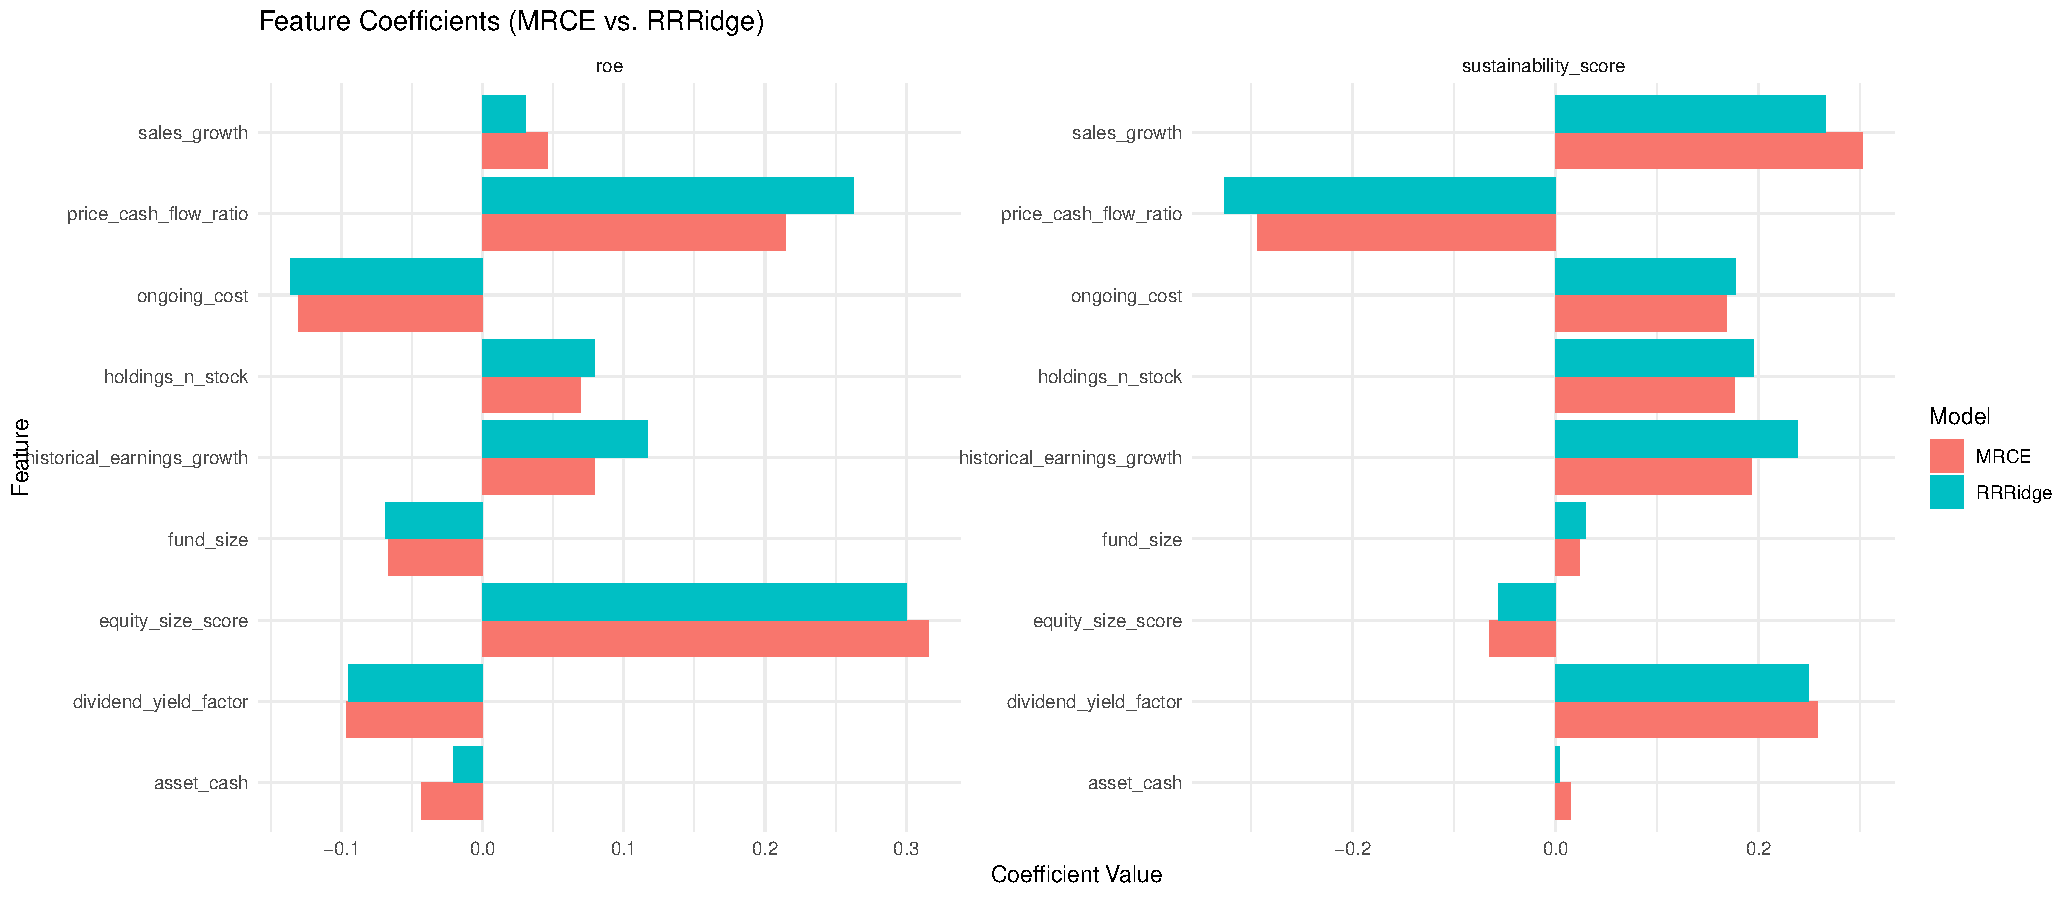
\includegraphics[width=0.9\linewidth]{MRCE vs. RRRR.pdf}
    \caption{MRCE vs RRRR Feature Contributions}
    \label{fig:MRCE vs RRRR}
\end{figure}

\noindent For ROE, both models identify \texttt{price\_cash\_flow\_ratio}, \texttt{category}, and \texttt{equity\_size\_score} as important predictors. However, MRCE applies stronger shrinkage to these variables because it estimates both the coefficient and inverse error covariance matrix simultaneously. As a result, \texttt{price\_cash\_flow\_ratio} has a much smaller coefficient in MRCE. \texttt{sales\_growth} has little influence in either model, while \texttt{asset\_cash} is slightly negative in MRCE but negligible in RRRR.

For the \texttt{sustainability\_score}, the differences between models are more noticeable. \texttt{sales \linebreak\_growth} is the strongest positive predictor in both cases, with MRCE assigning it a slightly larger coefficient. On the other hand, \texttt{historical\_earnings\_growth} has a strong positive effect in RRRR but is heavily shrunk in MRCE, likely due to concerns about multicollinearity, despite being addressed earlier in Chapter~\ref{EDA}. Interestingly, \texttt{category} receives a higher coefficient in MRCE, suggesting it emphasises the type of equity fund more. \texttt{equity\_size\_score} is close to zero in MRCE but still contributes to RRRR, and \texttt{price\_cash\_flow\_ratio} again has a larger absolute coefficient in RRRR.


% Multi-Output Gaussian Process Chapter
\chapter{Neural Networks}
The final chapter of this report will cover neural networks. It will start by explaining what a single-output neural network is and then move into a multi-output setting. Then, it will explain a Gaussian Process and a Multi-Output Gaussian Process. Ending with the methodology of a Multi-Output Gaussian Process Neural Network, a type of multi-output neural network, which will be explained and applied to the equity fund dataset.

\section{Theory}
While XGBoost refines predictions by iteratively improving decision trees, it still relies on rule-based partitioning of the feature space. Neural networks, however, take a different approach. They learn complex patterns through layers of interconnected neurons, which adapt to data.

\subsection{Introduction}
A neural network is a model which makes decisions like the human brain. It does this by a process similar to the way biological neurons work together to identify phenomena, weigh decisions and arrive at conclusions.\cite{ibm2024neuralnetworks}

Nodes are a building block of a neural network. Each node is a linear regression model with input data, weights, a bias (or threshold), and an output.\cite{ibm2024neuralnetworks} Within a neural network, there are a series of layers of nodes. The first of which is called the input layer and the last is called the output layer. The layers in between are called the hidden layers.

A Feed-Forward Neural Network (FFNN), otherwise known as a multi-layer perceptron, is a type of neural network whose vertices are numbered such that all connections go from a neuron (vertex) to one with a higher number. In other words, the information that enters all the nodes in the layers except the input is the sum of the information from those previous nodes. As information passes through the node, it is also changed by the weights of their respective prior corresponding nodes. The weights transform this information using the activation function. 

\noindent Each node in the network except the input layer is defined as:
\[
h_k^{(n)}(x) = \sigma_n \left( w_{k,0}^{(n)} + \sum_j w_{k,j}^{(n)} o_j^{(n-1)}(x) \right),
\]

\noindent where \( h_k^{(n)} \) is the linear combination of the \( k \)-th neuron in layer \( n \), \( \sigma_n \) is the activation function at layer \( n \), \( w_{k,0}^{(n)} \) is the bias term for the \( k \)-th neuron in layer \( n \), \( w_{k,j}^{(n)} \) is the weight from neuron \( j \) in layer \( n-1 \) to neuron \( k \) in layer \( n \), \( o_j^{(n-1)}(x) \) is the output of neuron \( j \) in the previous layer \( n-1 \), and \( o_j^{(0)}(x) = x_j \) are the input features for the input layer \( n = 1 \).

From what has been described, neural networks can capture linear models. They can be extended to capture potential non-linear relationships through the choice of activation function. Activation functions are non-increasing and are often sigmoids or threshold functions. Some examples of them include: the threshold sigmoid \ \(\sigma(\alpha) = 1 \ (\alpha > 0)\), the logistic sigmoid: \ \(\sigma(\alpha) = (1 + \exp(-\alpha))^{-1}\) and the rectified linear unit, RELU: \ \(\text{RELU}(\alpha) = \max(\alpha, 0)\).

\noindent Here is a graphic for a FFNN:
\begin{figure}[H]
    \centering
    \includegraphics[width=0.6\textwidth]{neuralnetwork.png}
    \caption{Neural Network Representation \cite{rosebrock2016neuralnetwork}}
    \label{fig:neuralnetwork}
\end{figure}

Neural networks can learn response inter-correlations between multiple outputs through their shared hidden layers. They capture correlations between these responses by using adaptive hidden units that were shared between the outputs.\cite{wilson2011gaussian} The shared hidden layers act as a latent space for the inputs, which is then transformed by weights.\cite{menet2023mimonets}

Each neuron in the output layer corresponds to one response variable. The weights connecting the hidden layer to the output neurons allow the FFNN also to learn output-specific mappings. These outputs are now coupled through a weight matrix, $W(x)$.

When training neural networks for a dataset, the choice of the loss function is critical in ensuring that all outputs are effectively optimised. A common approach is to compute the loss for each output individually and then aggregate the errors.\cite{menet2023mimonets} This can be done using the mean squared error or a weighted loss function to emphasise specific outputs.\cite{menet2023mimonets} The general form of the multi-output loss is:

\[
L(y, \hat{y}) = \frac{1}{p} \sum_{i=1}^{p} \left( y_i - \hat{y}_i \right)^2,
\]

\noindent where \( p \) represents the number of outputs, \( y_i \) is the actual value for the \( i \)-th output, and \( \hat{y}_i \) is the predicted value. For cases where outputs have different magnitudes or importance, a weighted loss can be applied:

\[
L(y, \hat{y}) = \frac{1}{p} \sum_{i=1}^{p} w_i \left( y_i - \hat{y}_i \right)^2,
\]

\noindent where \( w_i \) is the weight assigned to the \( i \)-th output. This approach ensures that higher-priority outputs receive greater attention during training.

\subsection{Multi-Output Neural Networks}
Multi-Output neural networks do not differ much to single-output neural networks unlike all the other models discussed in this report. However, they do bring their own benefits and drawbacks.

Training neural networks with multiple outputs introduces unique challenges, including gradient imbalance, where outputs with larger gradients dominate the optimisation process.\cite{menet2023mimonets} This can lead to poor performance for smaller-gradient outputs. Several techniques can mitigate this issue. 

\noindent The first of which is Gradient Clipping, which limits the magnitude of gradients during back-propagation to prevent a single output from dominating the learning process. Next, output-specific learning rates can also ensure optimisation is not rushed. Finally, batch normalisation, which involves normalising the activations in each layer, ensures gradients remain stable and uniform across all outputs.

The choice of activation function in the output layer depends on the type of regression problem. For continuous outputs, linear activation functions are typically used:

\[
o_j^{(n)}(x) = w_{k,j}^{(n)} o_j^{(n-1)}(x) + b_k^{(n)}
\]

However, sigmoid or softmax activation functions can be applied to bounded outputs (e.g., probabilities). For unbounded outputs, the Rectified Linear Unit (ReLU) activation is used due to its simplicity and effectiveness in learning non-linear patterns.

Regularisation helps prevent over-fitting in neural networks. This is especially important in multi-output settings where the network may over-fit one output at the expense of others. An example of this is L2 Regularisation, which penalises large weights in the output layer, effectively shrinking them during training:
    \[
    R(W) = \lambda \sum_{i,j} W_{i,j}^2
    \]
    where \( \lambda \) is the regularisation strength.\cite{menet2023mimonets}

Dropout is another regularisation method neural networks can use. It works by literally ‘dropping’ neurons out from internal layers during training to introduce noise, forcing the network to learn more relevant features. It can also be applied selectively to the output layer and used in MRR. Extending dropout by deactivating the hidden layer neurons ensures that no single output becomes over-fitted.

A key change to a standard Multi-Output Neural Network that I wanted to make was to introduce task-specific layers as well as the shared hidden layers because although we want the model to learn the responses using the same inputs so we consider their dependencies, what is important to consider is how dependent they are. \texttt{roe} and \texttt{sustainability\_score} have a -0.3171 correlation. So, giving them the exact same input nodes would lose some information.

Multi-output neural networks can provide insight into the relationships between outputs and features. However, they do not explicitly consider response intercorrelations. This lack of response correlation matrix consideration in the multi-output neural network makes it not usable for a lot of MRR. A Multi-Output Gaussian Process Neural Network, however, does consider this.

\section{Multi-Output Gaussian Process Neural Network}

\subsection{Gaussian Process}
First, let us define a Gaussian Process, which is a building block of a Multi-Output Gaussian Process (MOGP).

A Gaussian Process model is a probabilistic model over possible functions that fit a set of points.\cite{10360364} As a result, we can derive the means and variances to represent the function's maximum likelihood estimate and indicate prediction confidence, respectively.\cite{10360364}

A function, $f(x)$, is drawn from a Gaussian Process if for any finite set of input points $\mathbf{X} = \{\mathbf{x_1},...,\mathbf{x_n}\}$, the corresponding function values $\boldsymbol{f}(\mathbf{X}) = [f(\mathbf{x}_1),...,f(\mathbf{x}_n)]$ follows a multivariate normal distribution:

\[P(\boldsymbol{f}|\mathbf{X}) = \mathcal{N}(\boldsymbol{f}|\mathbf{m},\mathbf{K}),\]

\noindent where $\mathbf{m}(\mathbf{x})$ is the mean function and $\mathbf{K}(x,x')$ is the kernel function, which is the positive definite covariance between function values.\cite{10360364}

\noindent From here, we predict at new points $\mathbf{X_*}$ as $\boldsymbol{f(X_*)}$ for the joint distribution of $\boldsymbol{f}$ and $\boldsymbol{f_*}$:

\[
\begin{bmatrix} \boldsymbol{f} \\ \boldsymbol{f}_* \end{bmatrix} \sim \mathcal{N}
\left(
\begin{bmatrix} \mathbf{m}(\mathbf{X}) \\ \mathbf{m}(\mathbf{X}_*) \end{bmatrix},
\begin{bmatrix} \mathbf{K} & \mathbf{K}_* \\ \mathbf{K}_*^\top & \mathbf{K}_{**} \end{bmatrix}
\right),
\]

\noindent where $\mathbf{K} = K(\mathbf{X},\mathbf{X})$, $\mathbf{K_*} = K(\mathbf{X},\mathbf{X_*})$ and 
$\mathbf{K_{**}} = K(\mathbf{X_*},\mathbf{X_*})$ and with no observation, the mean, $(m(\mathbf{X},m(\mathbf{X_*}))=\mathbf{0}$.\cite{10360364}

This equation is the joint probability distribution $P(\boldsymbol{f}, \boldsymbol{f_*}|\mathbf{X},\mathbf{X_*})$ over $\boldsymbol{f}$ and $\boldsymbol{f_*}$ but this model is regression meaning only the conditional distribution $P(\boldsymbol{f_*}| \boldsymbol{f},\mathbf{X},\mathbf{X_*})$ is needed.\cite{10360364} The conditional distribution can be derived using the joint distribution, and it uses the marginal and conditional distributions of the multivariate normal theorem, which is explored further in Bishop et al. (2006). This proves the conditional distribution:

\[
\boldsymbol{f_*} |\boldsymbol{f},\mathbf{X},\mathbf{X_*} \sim \mathcal{N}(\mathbf{K}_*^\top\mathbf{K}^{-1}\boldsymbol{f}, \mathbf{K}_{**} - \mathbf{K}_*^\top\mathbf{K}^{-1}\mathbf{K}_*).
\]

\noindent The conditional distribution gives Gaussian Process regression's predictive equations:

\[
\bar{\boldsymbol{f_*}}|\mathbf{X},\mathbf{y},\mathbf{X}_* \sim \mathcal{N}(\bar{\boldsymbol{f_*}}, \text{Cov}(\boldsymbol{f}_*)),
\]

\noindent where $\bar{\boldsymbol{f_*}} = \mathbf{K}_*^\top (\mathbf{K}+\sigma_n^2 \mathbf{I})^{-1} \mathbf{y}$ and $\text{Cov}(\boldsymbol{f}_*) = \mathbf{K}_{**}-\mathbf{K}_*^\text{T}[\mathbf{K} + \sigma_n^2\mathbf{I}]^{-1}\mathbf{K}_*$.\cite{10360364}

\noindent The adjustment to $\mathbf{K}$ happens because of the noise we have to add to true function values in reality: $y = f(x) + \epsilon$, where $\epsilon$ is a standard independent and identically distributed Gaussian noise with variance $\sigma_n^2$.\cite{10360364} This adjusts the prior covariance to: $\mathbf{\Sigma_Y} = \mathbf{K} + \sigma_n^2\mathbf{I}$, which gives the previously defined predictive distribution.

\subsection{Multi-Output Gaussian Process Neural Networks}
Now Gaussian Processes have been set up, let us define a basic Multi-Output Gaussian Process (MOGP). This involves $L$ independent Gaussian processes $\{\boldsymbol{f}_{\ell}\}$ with $\ell = 1,\dots, L$, each with kernel $K_\ell$ and leads to the definition of the marginal probability of MOGP:\cite{blundell2015weight} 

\begin{equation}
    p(\mathbf{Y} | \mathbf{X}) = \int d\mathbf{M} p(\mathbf{M}) 
\prod_{\ell=1}^{L} d\boldsymbol{f}_\ell p(\boldsymbol{f}_\ell | \mathbf{X}) \times
\prod_{i=1}^{N} \mathcal{N} \big(y_i \mid \mathbf{M} \mathbf{F} (\mathbf{x}_i), \beta \big),
\label{MOGP}
\end{equation}


where $\mathbf{M}$ is a $D_Y \times L$ mixing matrix, $\mathbf{M}\mathbf{F}$, the covariance structure, is being matrix multiplied, and $p(\mathbf{M})$ is a unit Normal prior on $\mathbf{M}$.\cite{jankowiak2019neural}
Other covariance structures are possible for the Gaussian process, because owe are trying to uncover changes to the likelihoods, the model employs this basic pattern. For this reason, we use radial basis function kernels throughout.\cite{jankowiak2019neural}

Equation \ref{MOGP} can be extended by considering a model specified by its marginal likelihood as:

\begin{equation}
\int d\mathbf{M} p(\mathbf{M}) 
\prod_{\ell=1}^{L} d\boldsymbol{f}_\ell p(\boldsymbol{f}_\ell | \mathbf{X}) 
\prod_{i=1}^{N} \mathcal{N} \big(y_i \mid \mathbf{M} \sigma (\widetilde{\mathbf{M}} \mathbf{F} (\mathbf{x}_i)), \beta \big),
\label{MOGP NN}
\end{equation}

\noindent where $\mathbf{F}$ is passed through a neural network before it is used to compute the mean function for the likelihood.\cite{jankowiak2019neural} $\widetilde{\mathbf{M}}$ is a $D_H \times D_L$ matrix and $\mathbf{M}$ is a $D_Y\times D_H$ matrix, where $D_H$ is a new hyper-parameter which controls the number of `hidden units'.\cite{jankowiak2019neural} $\sigma(\cdot)$ is the activation function and $\mathbf{M}$ has a unit Normal prior. This is the mathematical framework of a MOGP Neural Network (NN). Now, let us go into how this actually generates and refines predictions.

%A MOGP NN does not contain an NN that is conditioned on the inputs as a subcomponent, which makes it less prone to overfitting to other types of NNs.

Practically, what will happen is, is that the neural network will come up with an initial prediction using its standard mechanisms. So, it uses forward and backward propagation to determine the optimal weights and biases for the most accurate initial prediction, $\mathbf{\hat{Y}}$. This prediction is then refined by the MOGP in the following way.

When a new data point, \(\mathbf{x}_*\), is provided for task \( l \), it is given by
\[
\bar{f}_l(\mathbf{x}_*) = \left( \mathbf{k}_l^f \otimes \mathbf{k}_*^x \right)^T \mathbf{\Sigma}^{-1} \mathbf{\hat{Y}},\quad
\mathbf{\Sigma} = \mathbf{K}^f \otimes \mathbf{K}^x + \mathbf{D \otimes I},
\]
\noindent where \(\otimes\) denotes the Kronecker product, \(\mathbf{k}_l^f\) selects the \(l^{\text{th}}\) column of \( \mathbf{K}^f \), \(\mathbf{k}_*^x\) is the vector of covariances between the test point \(\mathbf{x}_*\) and the training points, \( \mathbf{K}^x \) is the matrix of covariances between all pairs of training points, \( \mathbf{D} \) is an \( M \times M \) diagonal matrix in which the \((l,l)^{\text{th}}\) element is \( \sigma_l^2 \), and \( \mathbf{\Sigma} \) is an \( MN \times MN \) matrix with the covariances of the responses and predictors all in one.\cite{bonilla2007multi}
$\mathbf{K}^f= \mathbf{\Sigma_Y}$ so it is essential because it is what makes MOGP NN an MRR model. 

The predictor covariance matrix \(\mathbf{K}^x\) is computed using the radial basis function kernel:
\[
K^x(i,j) = \exp \left( -\frac{||X_i - X_j||^2}{2 \ell^2} \right),
\]
\noindent where $\ell$ is calculated by taking the median of all the pairwise Euclidean distances in the dataset and normalising by $\sqrt{2}$.\cite{bonilla2007multi}

The task covariance, or coregionalisation matrix, \(\mathbf{K}_f\), is estimated using the sample response covariance, $\mathbf{\Sigma_Y}$:
\vspace{-0.2cm}
\[
K_f(l, k) = \frac{1}{N} \sum_{i=1}^{N} (Y_{i,l} - \mu_l)(Y_{i,k} - \mu_k),
\]
\noindent where \(\mu_l\) is the mean response for each task. The noise variance matrix \(\mathbf{D}\) is then computed as the diagonals of the $\mathbf{K}_f$ matrix.\cite{bonilla2007multi} 

Finally, there is a potential issue of dimensionality but this is sorted by a shape restructuring of the neural network prediction from $N\times M$ to $MN\times1$.


\section{Application}

\subsection{Small-Scale Example}
We will apply the MOGP NN to this familiar dataset.
\setlength{\tabcolsep}{4pt} % Adjust column spacing
\begin{table}[H]
    \centering
    \begin{tabular}{|c|c|c|c|}
        \hline
        \( X_1 \): Hours Studied & \( X_2 \): Time Spent on Papers & \( Y_1 \): Math Scores & \( Y_2 \): Science Scores\\
        \hline
        5  & 2  & 78 & 80 \\
        7  & 3  & 85 & 79 \\
        8  & 4  & 88 & 88 \\
        3  & 1  & 65 & 70 \\
        10 & 5  & 92 & 74 \\
        \hline
    \end{tabular}
    \caption{Study Time vs. Exam Scores}
    \label{tab:study_scores7}
\end{table}
\noindent The first step is normalising all of the data.
We then define a two-layer neural network with a shared hidden layer and a task-specific layer to keep simplicity. See \ref{NN Visualisation} for the image. Although the neural network does learn response intercorrelation in the hidden layer, this is not explicit. As a result, let us assume that after forward and backward propagation, we have the following weight matrix and bias vector (to 2dp):
\[
\mathbf{W} =\begin{bmatrix}
    w_{11} & w_{12} & w_{h1} \\
    w_{21} & w_{22} & w_{h2}
\end{bmatrix}=\begin{bmatrix}
    1.40 & -0.72 & 0.70 \\
    -0.47 & 0.41 & 0.72
\end{bmatrix}, \quad \mathbf{b}=\begin{bmatrix}
   b_1 \\
    b_2\\
    b_{h1}\\
    b_{h2}
\end{bmatrix}=\begin{bmatrix}
   0.25 \\
    0\\
    0.53\\
    0.14
\end{bmatrix}.
\]
\noindent This gives the normalised inputs and neural network predictions as (to 2dp):
\begin{table}[H]
    \centering
    \begin{tabular}{|c| c | c| c|}
        \hline
        X$_1$: Hours Studied & X$_2$: Time Spent on Papers & 
        Y$_1$: Maths Score & Y$_2$: Science Score  \\
        \hline
        0.29  & 0.25  & 0.27  & 0.28  \\
        0.57  & 0.50   & 0.70  & -0.16  \\
        0.71  & 0.75  & 0.84  & -0.54  \\
        0.00  & 0.00  & 0.19  & 0.36  \\
        1.00  & 1.00  & 1.03  & -1.09  \\
        \hline
    \end{tabular}
    \caption{Normalised Maths and Science Scores}
    \label{tab:normalised_scores}
\end{table}
\noindent These values correspond to $\mathbf{\hat{Y}}$ in the MOGP notation. Now, we need to adjust these predictions.

%We now pass \( Z \) into a Multi-Output Gaussian Process: $Y \sim \mathcal{GP}(m(Z), K(Z, Z'))$, where \( m(Z) \) is the mean function and \( K(Z, Z') \) is the covariance function.
The first step involves calcaulting the input and response covariance matrices,  \(\mathbf{K}^x\) and  \(\mathbf{K}_f\).
The input covariance matrix \(\mathbf{K}^x\) is computed using the radial basis function kernel:
\[
K^x(i,j) = \exp \left( -\frac{||X_i - X_j||^2}{2 \ell^2} \right),
\]
\noindent where $\ell$ is calculated by taking the median of all the pairwise Euclidean distances in the dataset and normalising by $\sqrt{2}$. For simplicity, let us assume \(\ell = 2\). Here is how you compute $K^x(i,j)$ for 1 element: $(i,j)=(1,2)$. This manual computation gives:
\[
||X_1 - X_2||^2 = (0.29-0.25)^2 + (0.57-0.5)^2 = 0.0065.
\]

\noindent Therefore, $
K^x(1,2) = \exp \left( -\frac{0.0065}{2(2.5)^2} \right) \approx 1.00$.
The task covariance matrix, \(\mathbf{K}_f\), is estimated using the sample response covariance:
\vspace{-0.2cm}
\[
K^f(l, k) = \frac{1}{N} \sum_{i=1}^{N} (Y_{i,l} - \mu_l)(Y_{i,k} - \mu_k),
\]
\noindent where \(\mu_l\) is the mean response for each task:
\[
\mu_1 = \frac{0.27+0.70+0.84+0.19+1.03}{5} = 0.606
,\quad
\mu_2 = \frac{0.28-0.16-0.54+0.36-1.09}{5} = -0.23
\]
\noindent Plugging in for $\mathbf{K}_f$ gives:
\[\mathbf{K}^f =
\begin{bmatrix}
0.28 & -0.28 \\
-0.28 & 0.35
\end{bmatrix}
\]
\noindent The noise variance matrix \(\mathbf{D}\) is then computed as the diagonals of the full $\mathbf{K}_f$ matrix. 
Therefore, \(\mathbf{D}\) is:
\[
\mathbf{D} =
\begin{bmatrix}
0.28 & 0 \\
0 & 0.35
\end{bmatrix},
\]

The full covariance matrix, \(\mathbf{\Sigma}\), for the responses and the predictors, is then given by:
\[
\mathbf{\Sigma} = \mathbf{K}_f \otimes \mathbf{K}^x + \mathbf{D} \otimes \mathbf{I},
\]
\noindent which is a $10 \times 10$ matrix, so for simplicity, let us avoid using it and talk more abstractly. 
%see ... for further info
This matrix helps us to calculate the updated normalised prediction using:
\[
\bar{f}(\mathbf{x}_*) = (\mathbf{k}_l^f \otimes \mathbf{k}_*^x)^\top\mathbf{\Sigma}^{-1}\mathbf{\hat{Y}}.
\]
Here, we remember the potential issue of dimensionality is sorted by a shape restructuring of the neural network prediction from $5\times 2$ to $10\times1$.
Finally, this prediction will be in its normalised form, so the MOGP NN reverts the normalised predictions back to normal and then assess the ANRMSE.

\subsection{Code Explanation}
The code integrates a Neural Network (\texttt{Feature Extractor}) with a Multi-Output Gaussian Process (\texttt{MultiTaskGPModel}) to handle multi-task regression. The neural network extracts shared patterns from input features, while the Gaussian Process explicitly models dependencies between outputs using a coregionalisation matrix. A custom loss function ensures the predicted covariance structure aligns with actual relationships between outputs.

The neural network processes inputs through shared layers in \texttt{FeatureExtractor.forward()}, transforming them into a latent feature representation. Task-specific layers (\texttt{TaskHead.forward()}) then refine these representations, allowing the model to capture common structures while preserving flexibility for each task.

The Gaussian Process (GP) component models the outputs as a multivariate Gaussian distribution, capturing both uncertainty and inter-task correlations. It is implemented in \texttt{MultiTaskGPModel} using a constant mean function (\texttt{ConstantMean()}), an RBF kernel (\texttt{RBFKernel()}) for smooth variations, and a multitask covariance kernel (\texttt{MultitaskKernel()}) to structure dependencies between outputs.

A standard MSE loss function is used to monitor how accurate predictions are.

The model is trained using k-fold CV in \texttt{train\_model\_kfold()}, which splits the dataset into training and validation folds.
Then, it trains the neural network using \texttt{FeatureExtractor.train()}, optimising parameters via stochastic gradient descent.
Next, it passes transformed features into the Gaussian Process, optimising its hyperparameters through marginal log-likelihood maximisation (\texttt{gpytorch.mlls.ExactMarginalLogLikelihood()}).
Finally, it jointly updates both components to align the neural network representations with the Gaussian Process structure.

\subsection{Results}
The ANRMSE for the model is 0.411, indicating a reasonable fit, which is the best model. This value indicates the best fit, which makes sense because of how complex a MOGP NN is.

\begin{figure}[H]
    \centering
    % First image
    \begin{minipage}[b]{0.49\textwidth}
        \centering
        \includegraphics[width=\textwidth]{NN ROE FI.png} % Replace with your image path
    \end{minipage}
    \hfill
    % Second image
    \begin{minipage}[b]{0.49\textwidth}
        \centering
        \includegraphics[width=\textwidth]{NN SUS FI.png} % Replace with your image path
    \end{minipage}
    \caption{MOGP NN Feature Importance}
    \label{fig:sidebyside_minipage2}
\end{figure}

\noindent 
For return on equity, fund size, rating, sales growth, and risk rating are the most influential features. These features contribute heavily to the hidden layer activations in the neural network, shaping the learned representations. The GP component then refines these representations by modelling the covariance structure between outputs, leveraging correlations to improve predictions. Higher-importance features significantly reduce posterior variance, making predictions more stable and reliable.

For sustainability score, category, asset cash, and dividend yield factor play a dominant role. Since the Gaussian process integrates these features into a shared latent function space, their high importance indicates that they strongly influence the joint distribution of outputs. The neural network learns a nonlinear transformation of these features, which the Gaussian process then smooths through the RBF. This allows the model to fit the test data well while maintaining response intercorrelation.

In essence, highly ranked features act as strong priors in the network, guiding weight updates in the neural layers and refining the covariance estimation in the Gaussian process. This allows the model to balance assessing feature importance and accurate predictions.

Although Neural Networks have proven to be very effective when combined with Multi-Task Gaussian Processes, they come with some setbacks.
One major drawback is their dependency on large amounts of data. Neural networks require extensive labelled datasets to learn meaningful patterns, and without sufficient data, they are prone to overfitting or failing to fit test data effectively. 
Another significant limitation is their computational complexity. Training deep neural networks requires substantial computational power, often necessitating the use of specialised hardware such as GPUs or TPUs. The high memory requirements for storing weights and activations add to their resource intensity, making them expensive to train and deploy.


%Appendix of it...
\subsection{Multi-Output Gaussian Process Neural Network}
\subsubsection{Example Multi-Output Neural Network Visualisation}
\label{NN Visualisation}
\begin{figure}[H]
    \centering
    \includegraphics[width=0.5\linewidth]{Neural Network Diagram.png}
    \caption{Neural Network Example Diagram}
    \label{fig:NN e.g.}
\end{figure}


% Old summary of each chapter:
The remainder of this report is structured into a series of chapters that progressively build towards a comprehensive modelling and comparison of multiple-response regression methods.

Chapter 2 begins with Exploratory Data Analysis (EDA). The initial dataset includes both equity and bond funds with a high degree of missingness. This chapter focuses on cleaning and refining the dataset, defining the predictor variables, identifying relationships between the two response variables—return on equity (ROE) and sustainability score (SS)—and applying imputation techniques to address missing data.

Chapter 3 introduces the Multiple Response Linear Regression (MRLR) framework. It presents the core theory underlying MRLR and explains how it can be combined with Multiple Analysis of Variance (MANOVA) and stepwise selection to build interpretable models. Model fit is evaluated using both theoretical and empirical tools.

Chapter 4 progresses to shrinkage-based regression methods, including ridge regression and reduced rank regression. These methods are adapted to the multivariate setting and then applied to the dataset. Their performance is assessed to determine whether they offer improvements over the MRLR models.

Chapter 5 introduces non-linear modelling through Random Forests, including their adaptation to the multiple-response context. The chapter discusses the theoretical basis of multivariate random forests and evaluates their performance on the dataset.

Chapter 6 continues the non-linear modelling theme by examining XGBoost. This chapter outlines the necessary modifications for handling multiple response variables and evaluates the model using residual diagnostics and performance comparisons with random forests.

Chapter 7 introduces a neural network-based approach, specifically a multi-output Gaussian Process Neural Network. The chapter discusses its construction, theoretical motivation, and ability to capture complex relationships in the data.

Finally, Chapter 8 provides a conclusion, comparing the performance of all the modelling approaches applied. It identifies the most effective method for predicting ROE and SS, reflects on the findings, and discusses potential directions for future work.




% Old Challenges and Limitations:
In addition, multivariate techniques give meaningful results that need a large sample of data; otherwise, the results are meaningless due to high standard errors.\cite{jackson2018multivariate} There is more confidence in the results from a large sample rather than a small one. 

The performance of MRR models heavily depends on the availability of high-quality datasets with multiple correlated response variables. However, real-world datasets often contain missing values, noise, or imbalanced responses, which can affect model accuracy. Limited dataset diversity may also lead to overfitting, reducing the generalisability of findings across different domains.

There is often a trade-off between interpretability and predictive performance in MRR models. Linear models and shrinkage methods (e.g., ridge regression, LASSO) provide interpretable results but may struggle with complex, non-linear relationships. On the other hand, tree-based models and deep learning approaches can improve accuracy but often function as black boxes, making it difficult to extract meaningful insights from model coefficients.

Certain MRR models, particularly those involving covariance estimation, ensemble learning, or neural networks, require significant computational resources. As the number of predictors and response variables increases, training time and memory usage grow exponentially, posing scalability challenges. Efficient implementations and parallel computing techniques may be necessary to handle high-dimensional datasets effectively.

MRR models often assume low multicollinearity among predictors, but real-world data frequently violates this assumption. Strong correlations between predictors can lead to unstable coefficient estimates, particularly in traditional regression models. Additionally, high-dimensional datasets pose challenges, increasing the risk of overfitting. Dimensionality reduction techniques such as principal component regression can mitigate this issue, but they may also reduce model interpretability.

Many MRR methods involve complex hyperparameters, including regularisation strengths, number of latent components, or tree depth in ensemble models. Identifying the optimal hyperparameters requires extensive CV, grid search, or Bayesian optimisation, which can be computationally expensive. Additionally, hyper-parameter sensitivity may lead to instability in model performance, requiring careful tuning to ensure robust results.

% Previous Cholesky Gaussian XGBoost
\subsection{Cholesky-Gaussian XGBoost}
XGBoost uses Cholesky decomposition in multi-target regression to ensure that the covariance matrix remains positive definite while maintaining computational efficiency. During training, XGBoost fits trees not just for the mean of each target but also for the parameters of \( \mathbf{L} \). Instead of directly predicting covariance terms, the model learns the Cholesky-transformed values. The loss function used is the Negative Log-Likelihood of the multivariate Gaussian:

\begin{equation*}
-\log f(\mathbf{Y} | \boldsymbol{\mu}_{\mathbf{x}}, \Sigma_{\mathbf{x}}) =
\frac{ND}{2} \log (2\pi) + \frac{N}{2} \log |\Sigma_{\mathbf{x}}| 
+ \frac{1}{2} \sum_{i=1}^{N} (\mathbf{y}_i - \boldsymbol{\mu}_{\mathbf{x}})^\top 
\Sigma_{\mathbf{x}}^{-1} (\mathbf{y}_i - \boldsymbol{\mu}_{\mathbf{x}})    
\end{equation*}

\noindent The gradients and Hessians are computed with respect to the elements of \( \mathbf{L} \). By doing so, the optimisation process remains stable, avoiding issues that arise when directly estimating \( \mathbf{\Sigma}_x \), such as singularity or near-zero eigenvalues. Here is how to compute the gradients and Hessians.



% Low Rank Cholesky and Gaussian
\noindent Given the low-rank Cholesky decomposition, \( \mathbf{\Sigma}_{\mathbf{x}} = \mathbf{L} \mathbf{L}^\top \), the the negative log-likelihood gradient is:

\[
\frac{\partial \mathcal{L}}{\partial \mathbf{L}} = \mathbf{L}^{-T} - \mathbf{\Sigma}_{\mathbf{x}}^{-1} \mathbf{S}
\]

\noindent where:

\[
\mathbf{S} = \sum_{i=1}^{N} (\mathbf{y}_i - \boldsymbol{\mu}_{\mathbf{x}})(\mathbf{y}_i - \boldsymbol{\mu}_{\mathbf{x}})^\top
\]

\noindent is the scatter matrix.\cite{tan2021analytic} And, the Hessian (second derivative) of the negative log-likelihood with respect to \( \mathbf{L} \) is:

\[
\mathbf{H} = \mathbf{L}^{-T} \otimes \mathbf{L}^{-1} + (\mathbf{\Sigma}_{\mathbf{x}}^{-1} \otimes \mathbf{\Sigma}_{\mathbf{x}}^{-1}) \mathbf{S}
\]

\noindent where \( \otimes \) denotes the Kronecker product.\cite{tan2021analytic} For computational efficiency, an approximation is often used:
$
\mathbf{H} \approx \mathbf{L}^{-T} \otimes \mathbf{L}^{-1},
$ which is diagonal-dominant.\cite{tan2021analytic}




% Low Rank Cholesky Decomposition
\noindent In addition to covariance matrix reparametrisation, the Cholesky decomposition is also computationally efficient since only the determinant of a triangular matrix needs to be calculated.\cite{Salinas2019}

While efficient for low to medium dimensions of \( D \), the computational cost of the Cholesky decomposition becomes prohibitive in high-dimensional settings. To reduce the computational overhead, the covariance matrix \( \boldsymbol{\Sigma} \) can be approximated via the sum of a diagonal matrix \( \mathbf{K} \in \mathbb{R}^{D \times D}_+ \) and an unrestricted low-rank matrix \( \mathbf{V} \in \mathbb{R}^{D \times r} \):

\[
\mathbf{\Sigma} = \mathbf{K} + \mathbf{V} \mathbf{V}^{T}
= \begin{bmatrix}
\exp(K_1) & \dots & 0 \\
\vdots & \ddots & \vdots \\
0 & \dots & \exp(K_D)
\end{bmatrix}
+ 
\begin{bmatrix}
V_1 \\
\vdots \\
V_D
\end{bmatrix}
\begin{bmatrix}
V_1 \\
\vdots \\
V_D
\end{bmatrix}^{T}
\]

\noindent where $\exp(\cdot)$ ensures all diagonal entries of $\mathbf{K}$ to be strictly positive and the rank parameter $r$ governs approximation quality.\cite{marz2022multi} The computational efficiency of this approach results from the fact that the rank parameter $r \ll D$ can typically be chosen much smaller than the number of responses, $D$.\cite{Salinas2019}

% Multi-Output XGBoost 
\subsection{Multi-Output XGBoost}
XG Boost is primarily designed for single-response regression. However, it can handle MRR by incorporating random output projections. XGBoost in MRR is very similar to single-response.

Here is a standard multi-output XGBoost objective function extended to sum over all response dimensions:
\begin{equation*}
\mathcal{L}(\phi) = \sum_{i=1}^n \sum_{d=1}^D l(y_{id}, \hat{y}_{id}) + \sum_{t=1}^\top \Omega(f_t),
\end{equation*}

\noindent where $y_{id}$ and $\hat{y}_{id}$ are the observed and predicted values for target $d$ of instance $i$.\cite{9158536}

\noindent During each boosting iteration, a tree is fit to the joint residuals of all targets, capturing interactions between them. The split gain is computed by summing contributions from all response dimensions:

\begin{equation*}
\text{Gain} = \frac{1}{2} \left[ \sum_{d=1}^D \left( \frac{G_{Ld}^2}{H_{Ld} + \lambda} + \frac{G_{Rd}^2}{H_{Rd} + \lambda} - \frac{(G_{Ld} + G_{Rd})^2}{H_{Ld} + H_{Rd} + \lambda} \right) \right] - \gamma,
\end{equation*}

\noindent where $G_{Ld}, H_{Ld}$ and $G_{Rd}, H_{Rd}$ represent the gradients and Hessians for the left and right child nodes, respectively.\cite{9158536} This is similar to the single response case, but the sum is taken over all the responses.

Here is a visualisation of the Multi-Output XGBoost from left to right using simulated data:

\begin{figure}[H]
    \centering
    \begin{minipage}{0.49\textwidth}
        \centering
        \includegraphics[width=\linewidth]{XGBoost_Tree_Response_1.png}
    \end{minipage}
    \hfill
    \begin{minipage}{0.49\textwidth}
        \centering
        \includegraphics[width=\linewidth]{XGBoost_Tree_Response_2.png}
    \end{minipage}
    \caption{An Example of Multi-Output XGBoost in Action}
\end{figure}

\noindent However, standard multi-output XGBoost has a glaring problem. Like standard MRFs, it does not inherently consider response intercorrelation. This can be addressed by extending this method.


% Old Cholesky Decomposition XGBoost example
\noindent We assume that \( \mathbf{Y} | \mathbf{X} \sim \mathcal{N}(\mathbf{\mu}(X), \mathbf{\Sigma}(X)) \), where: \( \mathbf{\mu}(X) \) represents the conditional mean predictions, modelled using XGBoost and \( \mathbf{\Sigma}(X) \) represents the covariance structure, modelled using a low-rank Cholesky decomposition.

XGBoost starts with a base prediction, typically the mean of each target variable:

\[
\mu_1^0 = \frac{78 + 85 + 88 + 65 + 92}{5} = 81.6, \quad
\mu_2^0 = \frac{74 + 81 + 86 + 62 + 90}{5} = 78.6
\]

Thus, the initial predictions for both targets are:

\[
\hat{Y}_1^0 = 81.6, \quad \hat{Y}_2^0 = 78.6
\]

For all data points, this means the residuals are:

\[
\mathbf{r}_1 = Y_1 - \hat{Y}_1^0 =
\begin{bmatrix}
-3.6 \\
3.4 \\
6.4 \\
-16.6 \\
10.4
\end{bmatrix},
\quad
\mathbf{r}_2 = Y_2 - \hat{Y}_2^0 =
\begin{bmatrix}
-4.6 \\
2.4 \\
7.4 \\
-16.6 \\
11.4
\end{bmatrix}
\]

\noindent XGBoost fits decision trees to predict the residuals \( \mathbf{r}_1 \) and \( \mathbf{r}_2 \). For example, if we split at \( X_1 = 6 \):

\begin{itemize}
    \item Left group (\( X_1 \leq 6 \)): Mean residual = \( -10.1 \)
    \item Right group (\( X_1 > 6 \)): Mean residual = \( 6.73 \)
\end{itemize}

\noindent Predictions are updated by: $\hat{Y}_1^1 = \hat{Y}_1^0 + \eta \cdot T_1(X)$,
where \( \eta = 0.1 \) is the learning rate, yielding:

\[
\hat{Y}_1^1 =
\begin{cases}
81.6 + 0.1 \cdot (-10.1) = 80.59, & X_1 \leq 6 \\
81.6 + 0.1 \cdot (6.73) = 82.27, & X_1 > 6
\end{cases}
\]

\noindent A similar process applies for \( \mathbf{r}_2 \), leading to:

\[
\hat{Y}_2^1 =
\begin{cases}
78.6 + 0.1 \cdot (-10.6) = 77.54, & X_2 \leq 2.5 \\
78.6 + 0.1 \cdot (6.73) = 79.27, & X_2 > 2.5
\end{cases}
\]

\noindent The next step is to estimate the Covariance Matrix Using Low-Rank Cholesky in the first iteration. Instead of predicting \( \mathbf{\Sigma}(X) \) directly, we estimate its Cholesky decomposition:

\[
\mathbf{L} =
\begin{bmatrix}
\ell_{11} & 0 \\
\ell_{21} & \ell_{22}
\end{bmatrix}
\]

\noindent Applying Cholesky decomposition to the empirical covariance matrix:

\[
\mathbf{\Sigma} =
\begin{bmatrix}
140.7 & 144.6 \\
144.6 & 149.2
\end{bmatrix}
\]

\noindent Solving for \( \mathbf{L} \):

\[
\ell_{11} = \sqrt{140.7} \approx 11.86, \quad
\ell_{21} = \frac{144.6}{11.86} \approx 12.19, \quad
\ell_{22} = \sqrt{149.2 - (12.19)^2} \approx 2.83
\]

\noindent XGBoost then fits trees to predict: $\ell_{11}(X), \quad \ell_{21}(X), \quad \ell_{22}(X)$. After the first iteration, the covariance matrix is reconstructed as: $\mathbf{\Sigma} = \mathbf{L} \mathbf{L}^\top$.

\noindent Now repeat this step for the next iteration by computing new residuals and fitting new XGBoost trees for \( \hat{Y}_1, \hat{Y}_2 \). Then, fitting XGBoost trees for \( \ell_{11}, \ell_{21}, \ell_{22} \). And, finally, updating \( \mathbf{\Sigma}(X) = \mathbf{L} \mathbf{L}^\top \) and ensure it remains positive definite.

Iteration 1 reduces residual error by fitting trees to predict corrections.
Then, Iteration 2 refines the mean and covariance predictions. The covariance matrix remains positive definite by optimizing its Cholesky factors.
This process continues until convergence. 


% Kalman Filter...
However, rather than using this mean directly, our implementation further adjusts the predicted mean using a correction to account for the response covariances. This adjustment is given by:
\vspace{-0.1cm}
\begin{equation}
    \mathbf{Y}^* = \hat{\mathbf{Y}}^* + \mathbf{W} (\mathbf{{Y}}_{\text{OOB}} - \hat{\mathbf{Y}}^*),
    \label{adjust_mean}
\end{equation}

\noindent where \( \mathbf{W} \) is the precision matrix computed as:
$\mathbf{W} = (\hat{\mathbf{\Sigma}}^* + \lambda \mathbf{I})^{-1}$ and $\mathbf{{Y}}_{\text{OOB}}$ is all the observations at said node. This step ensures that the predicted mean is refined by incorporating information from the covariance structure, which makes it suitable for MRR. This refinement comes from the Kalman Filter which is predominantly used in Dynamical Systems for trajectory optimisation.\cite{ghysels2018applied} 

The Kalman Filter has 2 key stages: the prediction and update steps. The prediction step estimates the next state before considering previous observations:
\vspace{-0.2cm}
\begin{equation*}
    \hat{x}_{k|k-1} = F_k \hat{x}_{k-1|k-1} + B_k u_k,
\end{equation*}
where $F_k$ is the {state transition matrix} that models how the state evolves over time, $\hat{x}_{k-1|k-1}$ is the {previous updated state estimate}, $B_k$ is the {control input model} that defines how external inputs affect the state and $u_k$ is the {control input} applied at time $k$.\cite{faragher2012understanding} In CRRF, this corresponds to the prior response mean, $\mathbf{\hat{Y}}^*$, before adjustments.
The Kalman Filter also updates the response covariance matrix, but this is not necessary for CRRF as our focus is on updating the response means and the covariance $\hat{\mathbf{\Sigma}}_\mathbf{Y}^*$ is already estimated from the oob samples. See \ref{Kalman Filter Covariance Update} for more on this.

The next step is the update, which breaks down into 3 key parts and it corrects the prior response mean prediction. The first step is adjusting the residuals:
\vspace{-0.2cm}
\begin{equation*}
    \tilde{y}_k = z_k - H_k \hat{x}_{k|k-1}
\end{equation*}
where $\tilde{y}_k$ is the residual, the difference between the observed and predicted values, $z_k$ is the {new measurement} received at time $k$, and $H_k$ is the {observation matrix} that maps the state to the measurement space.\cite{faragher2012understanding} In CRRF, $H_k = \mathbf{I}$ since responses are directly observed and $z_k=\mathbf{\bar{Y}}_{\text{OOB}}$.

The next step is correcting the covariance to adjust for noise, $S_k$. For CRRF, this involves adding the regularisation term $\lambda \mathbf{I}$.

\noindent Finally, this all comes together in the Kalman Gain formula:
\begin{equation*}
    K_k = P_{k|k-1} H_k^T S_k^{-1}
\end{equation*}
where $P_{k|k-1}$ is the predicted covariance matrix before the update.\cite{faragher2012understanding} $K_k$ is the {Kalman gain}, determining how much weight is assigned to the new measurement.\cite{faragher2012understanding} In CRRF, this corresponds to the precision-weighted correction matrix: $\mathbf{W} = (\hat{\mathbf{\Sigma}}^* + \lambda \mathbf{I})^{-1}.$

These prior steps contribute to the whole state update. \begin{equation*}
    \hat{x}_{k|k} = \hat{x}_{k|k-1} + K_k \tilde{y}_k
\end{equation*}
where $\hat{x}_{k|k}$ is the {updated state estimate} incorporating the new measurement, the correction term $K_k \tilde{y}_k$ ensures the update balances prior information with new data.\cite{faragher2012understanding} In CRRF, the equivalent update formula is \ref{adjust_mean}.

\noindent See \ref{Kalman Filter Proof} for the full derivation of the Kalman Filter.


% Old MANOVA Stepwise Selection Explanation
This was broken down into a few functions to make the final function simpler. Firstly, a \texttt{calculate\_anrmse} function was made to determine model fit. Then, two additional functions were made: \texttt{add\_predictors} and \texttt{remove\_predictors}.

The \texttt{add\_predictors} function evaluates the effect of adding each remaining predictor to the regression model. It iterates over all available predictors that have not yet been selected and examines their effect by calculating the difference between the Wilks' Lambda values before and after adding said predictor. Differences are taken because the desired result is the largest drop in Wilks' Lambda value as specified by Sequential MANOVA. The models that have been tested and their respective Wilks' Lambda value differences are then stored in 2 separate lists, and the model with the largest difference is used next in the stepwise selection process. 

For each predictor being tested, a new multivariate regression model is constructed using the existing selected predictors along with the new candidate predictor. Let us look at an example of this: 
\[\text{cbind}(y_1, y_2) \sim x_1 + x_2 + x_3,\]
\noindent where \( y_1 \) and \( y_2 \) are the response variables \texttt{roe} and \texttt{sustainability\_score}, respectively, and \( x_1, x_2, x_3 \) are the selected predictors, with \( x_3 \) being the new candidate predictor. 

Once the model is built, a Wilks' Lambda MANOVA Test is performed. The corresponding Wilks' Lambda value is extracted from the MANOVA summary, and the difference is calculated as:
$
\Lambda_{j} - \Lambda_{j+1},
$
\noindent where $\Lambda_{j}$ is the Wilks' Lambda value for $\text{cbind}(y_1, y_2) \sim x_1 + x_2$ and $\Lambda_{j+1}$ is the Wilks' Lambda value for $\text{cbind}(y_1, y_2) \sim x_1 + x_2 + x_3$. Finally, the function stores the model and the Wilks' Lambda difference in 2 separate lists. After this, a new model is tested but using $x_4$ as the new candidate predictor instead of $x_3$, giving:

\[
\text{cbind}(y_1, y_2) \sim x_1 + x_2 + x_4,
\]

The $x_i$ that gives the largest Wilks' Lambda value is stored, and then the next model evaluated is $\text{cbind}(y_1, y_2) \sim x_1 + x_2 + x_i$ and we iterate through the remaining predictors again. All of these models that gave the largest Wilks' Lambda difference are then evaluated using the ANRMSE and the model with the lowest ANRMSE is taken.

The \texttt{remove\_predictors} function evaluates the effect of removing each selected predictor from the current model. This function ensures that only predictors that significantly impact the response variation remain in the model. It iterates over all currently selected predictors and temporarily excludes each predictor one at a time to assess its effect on model performance. For each exclusion, a new multivariate regression model is constructed using the remaining predictors. Similar to the \texttt{add\_predictors} function, this function performs a MANOVA using Wilks' Lambda test to determine the significance of each predictor. The function then returns a list of candidate models, each with its associated Wilks' Lambda difference and evaluates them using the ANRMSE as before.


The \texttt{stepwise\_multivariate} function brings this all together by performing stepwise selection for a multivariate regression model, specifically to predict the response variables \texttt{roe} and \texttt{sustainability\linebreak\_score}. It uses $k$-fold cross-validation (CV) to assess the predictive accuracy of the final selected model.

If the selection method is set to \texttt{"forward"}, the function starts with an empty set of predictors. Otherwise, it begins with all predictors included. If the method is \texttt{"forward"} or \texttt{"bidirectional"}, the function calls \texttt{add\_predictors} to evaluate the inclusion of each remaining predictor. If the method is \texttt{"backward"} or \texttt{"bidirectional"}, the function calls \texttt{remove\_predictors} to evaluate the exclusion of each selected predictor. The predictor with the most significant impact, as determined by the largest Wilks' Lambda difference, is either added or removed from the model. The selection process continues until no further improvement is observed. If two consecutive iterations fail to improve the model, meaning no predictors are added or removed, the selection process terminates.

\noindent To ensure that the selected model performs well on unseen data, the function performs $k$-fold CV. The dataset is divided into $k$ equal-sized folds using the \texttt{createFolds} function. For each fold, the model is trained using the remaining $k-1$ folds, and predictions are made on the held-out test fold. The NRMSE is computed separately for \texttt{roe} and \texttt{sustainability\_score}. After iterating through all $k$ folds, the final mean NRMSE is computed as the average of the individual NRMSE values for \texttt{roe} and \texttt{sustainability\_score}. 

%% Forward, Backward or Bi-directional
It follows one of three approaches: forward selection, backward elimination, or a combination of both: bidirectional selection. In forward selection, the function starts with an empty model and iteratively adds predictors that significantly improve it. In backward selection, the function starts with all predictors included and iteratively removes those that do not meaningfully contribute to predicting the response variables. Bidirectional selection combines both approaches, allowing predictors to be added or removed at each step depending on the Wilks' Lambda differences.

%%Extra MANOVA Info:
Wilks' Lambda also allows MANOVA to test the overall effect of an independent variable on a multivariate response. Instead of testing each dependent variable separately, it examines whether any linear combination of the dependent variables differs significantly between groups. This multivariate approach can detect group differences that may not be evident in individual ANOVA tests.\cite{Newsom2024MANOVA}

$\mathbf{W}$ and $\mathbf{T}$ are variance-covariance matrices, and their off-diagonal elements capture the covariation between response variables.

%% Former Introduction:
This report delves into the theory of different regression models and compares their performance on a Kaggle dataset. This dataset consists of equity funds, and the variables being modelled are return on equity and sustainability score against other fund features.
\\
\newline
\textbf{Chapter 2}: Exploratory Data Analysis - the master dataset consists of a mixture of equity and bond funds and a lot of missing data. This chapter involves cleaning and simplifying the dataset, defining the remaining predictors, understanding underlying relationships in the response variables and then imputing missing values.
\\
\newline
\textbf{Chapter 3} Multiple Response Regression - this gives a basic outline of multiple response regression and its underlying theories. Then, multiple-response stepwise selection methods are combined with MANOVA and applied, and their fit is analysed.
\\
\newline
\textbf{Chapter 4}: Shrinkage Methods - now, there is a progression to continuous regression methods and how they are adapted to the multivariate case. They are also applied and evaluated on the dataset, and the best among them is decided.
\\
\newline
\textbf{Chapter 5}: Random Forest Regression - the theory behind this method is introduced, and how now non-linear regression methods can apply to the dataset. Its adjustment to the multivariate case will be explained, and how well it models the data will be tested.
\\
\newline
\textbf{Chapter 6}: XG Boost - this is another non-linear approach which will be looked at for this dataset through residual evaluation. This will compare it to the random forest.
\\
\newline
\textbf{Chapter 7}: Neural Networks -are the final regression model that will be covered. They bring a whole new approach to modelling the dataset, and it introduces a complexity to understanding equity funds.
\\
\newline
\textbf{Chapter 8}: Conclusion - this will be a final comparison of all the regression models in the dataset, and it will ultimately decide which one is the best fit. Also, the conclusion will explain what further analysis could be done in this report.


%% XGBoost Missing Data
Although the data here has no missing data due to the initial exploratory data analysis, XGBoost can efficiently handle missing and sparse data through a sparsity-aware split-finding algorithm.\cite{chen2016xgboost} During tree construction, XGBoost learns the optimal default direction for missing values, reducing the need for data imputation. The split-finding process is defined as:

\begin{equation*}
f(x_i) = \begin{cases}
f_{\text{left}}(x_i) & \text{if } q_j \neq \text{missing} \\
f_{\text{default}}(x_i) & \text{if } q_j = \text{missing}
\end{cases}
\end{equation*}
This allows XGBoost to scale linearly with the number of non-missing entries. \cite{chen2016xgboost}

%% RRRR Intercorrelation Explanation
 This comes from first considering the empirical covariance of the responses: $\operatorname{Cov}(\mathbf{Y}) = \frac{1}{N} \mathbf{Y}^T \mathbf{Y}.$ If we perform SVD on \( \mathbf{Y} \) using
$\mathbf{Y} = \mathbf{U}_Y \mathbf{D}_Y \mathbf{V}_Y^T,$
then the covariance of \( \mathbf{Y} \) can be rewritten as:

\[
\operatorname{Cov}(\mathbf{Y}) = \frac{1}{N} \mathbf{V}_Y \mathbf{D}_Y^2 \mathbf{V}_Y^T.
\]

\noindent This shows us that the eigenvectors of \( \operatorname{Cov}(\mathbf{Y}) \) are given by \( \mathbf{V}_Y \). Eigenvectors define the principal correlated response directions, and the right singular vectors \( \mathbf{V}_Y \) correspond to the principal components of the response covariance matrix. The right singular vectors \( \mathbf{v}_i \) of \( \mathbf{Y}^*_R \) will approximate those of \( \mathbf{Y} \),  especially in the low-rank setting as it is its ridge prediction. Thus, \( \mathbf{v}_i \) in SVD of \( \mathbf{Y}^*_R \) captures response correlation structure.

%% XGBoost Old Results:
This code demonstrates the use of XGBoost to perform multi-output regression, predicting two target variables: \texttt{roe} and \texttt{sustainability\_score}. The model uses the \texttt{MultiOutputRegressor} wrapper from Scikit-Learn to enable the XGBoost model to predict multiple outputs simultaneously. 

The necessary Python libraries are imported at the beginning:
\texttt{pandas} are used for data manipulation, \texttt{xgboost} for modelling, \texttt{scikit-learn} provides tools for splitting data, evaluating model performance, and handling multi-output regression and finally, \texttt{numpy} is used for numerical operations.
A random seed is used here, too, like for random forest.

The dataset \texttt{clean.csv} is loaded into a Pandas DataFrame, and then the categorical columns (\texttt{rating}, \texttt{risk\_rating}, \texttt{category}) are frequency encoded by mapping the count of each category to the corresponding feature values like before. The feature matrix \( X \) and target matrix \( y \) are then defined by dropping and selecting relevant columns. \texttt{X} contains the predictor variables, while \texttt{y} contains the two target variables to be predicted.

Next, the dataset is split into training and testing sets (an 80/20 split) to evaluate model performance on unseen data. The XGBoost model can now be trained and tested.

An XGBoost regressor is initialised with specific hyper-parameters: \newline \texttt{objective='reg:squarederror'}, which specifies the regression objective, \newline \texttt{n\_estimators=100} sets the number of boosting rounds, \texttt{max\_depth=6} defines the maximum depth of each tree, \texttt{learning\_rate=0.1} controls the step size during boosting, and \texttt{random\_state=seed} ensures reproducibility.

Since XGBoost does not automatically handle multiple target variables, \linebreak \texttt{MultiOutputRegressor} is used to wrap the base model. This enables the model to predict numerous outputs by fitting one regressor per target. Then, the model is trained on the training data and predictions are made on the test set. Finally, model performance is evaluated using the Root Squared Residual (RSR) for each response variable, as done for the other models in this report.

\subsection{Results}
The \texttt{roe} RSR  was 0.313, suggesting that the model predicts ROE relatively well, as the RSR is quite low, implying the residuals are small compared to the variation in the data. The \texttt{sustainability\_score} RSR was 0.462. This value is higher, indicating that the model has more difficulty predicting sustainability scores accurately. The residuals are larger relative to the variability in the target. An average RSR of 0.387 across the two targets suggests overall decent performance. While not perfect, this value indicates that the model captures patterns in the data but leaves room for improvement, particularly for the sustainability score.

A SHAP plot is portrayed to understand the feature contribution to predictions:

\begin{figure}[ht]
    \centering
    % SHAP Plot for ROE
    \begin{subfigure}{0.45\textwidth}
        \centering
        \includegraphics[width=\textwidth]{xg_shap_roe.png}
        \subcaption{SHAP values for Return on Equity (ROE).}
        \label{fig:xg_shap_roe}
    \end{subfigure}
    \hfill
    % SHAP Plot for Sustainability Score
    \begin{subfigure}{0.45\textwidth}
        \centering
        \includegraphics[width=\textwidth]{xg_shap_sus.png}
        \subcaption{SHAP values for Sustainability Score.}
        \label{fig:xg_shap_sus}
    \end{subfigure}
    \caption{SHAP values illustrating feature impact on ROE and Sustainability Score.}
    \label{fig:xg_shap_plots}
\end{figure}

\noindent From Figure \ref{fig:xg_shap_roe}, it is evident that price\_cash\_flow\_ratio, dividend\_yield\_factor, and category are the most influential features affecting ROE. High values of price\_cash\_flow\_ratio and dividend\_yield\_factor tend to increase ROE, as indicated by the clustering of red dots on the positive side of the x-axis. Conversely, lower values of these features generally contribute to a reduction in ROE. The feature category also plays a significant role, with variations in its values leading to substantial shifts in the prediction.

The features historical\_earnings\_growth and equity\_size\_score exhibit wide spreads of SHAP values, suggesting considerable variability in their influence across different observations. This variability indicates that the impact of these features is not uniform and may depend on complex interactions with other variables. Similarly, ongoing\_cost and sales\_growth show that lower values negatively affect ROE, as reflected by the concentration of blue dots on the negative side of the plot. Certain features, such as fund\_size and asset\_cash, display relatively narrow distributions of SHAP values. This indicates that while these features have a consistent impact across the dataset, their overall contribution to ROE is more negligible compared to more dominant features. Despite their limited influence, these features still play a role in refining the model’s accuracy.

Category, holdings\_n\_stock, and price\_cash\_flow\_ratio emerge as the most influential features. High values of category and holdings\_n\_stock positively contribute to sustainability score predictions, while low values lead to reduced predictions.

Sales\_growth and historical\_earnings\_growth show wide spreads, suggesting significant variability in their effects across observations. Ongoing\_cost and dividend\_yield\_factor demonstrate consistent adverse effects when their values are low. Conversely, asset\_cash, fund\_size, and rating display limited yet consistent influence, indicating that while their overall contributions are small, they maintain predictive significance across the dataset.

The overlapping colours along the x-axis for both plots highlight the potential for non-linear relationships and intricate feature interactions. This variability suggests that the influence of specific features may be condition-dependent, reinforcing the importance of further investigation into these interactions.

A feature plot is also displayed again to show the contribution of specific predictors to the xgboost model:

\begin{figure}[H]
    \centering
    \includegraphics[width=0.9\textwidth]{xgboostfeatureimportance.png}
    \caption{XG Boost Feature Importance}
    \label{fig:xgboostfeatureimportance}
\end{figure}

\noindent The feature importance plots for the XGBoost model, predicting \texttt{roe} and \texttt{sustainability\linebreak \_score}, highlight the relative influence of various predictor variables. For the \texttt{roe} model, the most dominant feature is the \texttt{price\_cash\_flow\_ratio}, which shows a much larger importance compared to other variables. This indicates that cash flow relative to price plays a crucial role in determining return on equity. Following this, features such as \texttt{equity\_size\_score} and \texttt{dividend\_yield\_factor} also contribute significantly, though their importance is notably smaller. Additional variables, including \texttt{ongoing\_cost}, \linebreak \texttt{historical\_earnings\_growth}, and \texttt{sales\_growth}, provide further predictive value, but at a reduced scale.

In contrast, the \texttt{sustainability\_score} model attributes the highest importance to \texttt{dividend\_yield\_factor}, suggesting that dividend performance is a key determinant of sustainability. \texttt{Ongoing\_cost} and \texttt{holdings\_n\_stock} follow closely, reinforcing the idea that ongoing expenses and stock holdings shape the sustainability profile of an entity. Other influential factors include \texttt{category} and \texttt{price\_cash\_flow\_ratio}, although their contribution is less pronounced. 

Despite differences in dominant features, both models reveal a shared set of impactful variables, including \texttt{ongoing\_cost} and \texttt{sales\_growth}, indicating their broad relevance across financial and sustainability outcomes. The presence of categorical factors such as \texttt{risk\_rating} and \texttt{category} highlights the role of qualitative measures in predicting both target variables. 

These results suggest that while certain variables are critical for specific targets, the overlap in feature importance underscores a broader relationship between financial performance and sustainability metrics. The findings can help refine decision-making processes by emphasising key drivers tailored to each objective.


\begin{figure}[H]
    \centering
    \includegraphics[width=0.8\textwidth]{learningcurve.png}
    \caption{XG Boost Learning Curve}
    \label{fig:learningcurve}
\end{figure}

\noindent The plot illustrates the Average Root Squared Residual (ARSR) learning curve for an XGBoost model trained to predict two target variables: \texttt{roe} and \texttt{sustainability\_score}. The x-axis represents the number of boosting rounds, while the y-axis shows the ARSR values calculated for the test set. 

The downward trajectory of the curve indicates a consistent reduction in prediction error as the boosting rounds progress. Initially, during the early boosting rounds, the ARSR decreases rapidly, suggesting that the model is learning key patterns in the data and making significant performance gains. This phase demonstrates the model's ability to capture essential relationships between features and the target variables efficiently.

As the number of boosting rounds increases, the rate of ARSR reduction slows, and the curve begins to flatten. This plateau suggests diminishing returns from additional boosting, implying that the model is nearing its optimal performance. Despite further boosting, the marginal improvement in ARSR becomes smaller, reflecting the model's stability and reduced error.

The absence of significant fluctuations or increases in the ARSR throughout the boosting process indicates that the model is now over-fitting the training data. This smooth convergence reflects the model's ability to generalise well to unseen data, contributing to reliable predictions for both \texttt{roe} and \texttt{sustainability\_score}.

%% Random Forest Old Information:
This chapter has looked at single-response regression so far. Multivariate Regression Trees (MRTs), as introduced by De'ath (2002), are an extension of CART to handle several response variables.\cite{questier2005cart} MRTs split a response matrix into clusters based on thresholds of explanatory variables. This approach allows MRT to model complex, multivariate relationships by partitioning the data in a way that accounts for interactions between explanatory and response variables. Unlike single-response regression trees, MRTs highlight local data structures.\cite{qcbs_workshop}

\noindent MRTs are constructed similarly to CARTs, but they require criteria that account for the joint distribution of multiple response variables. The impurity measure in MRT minimises the total within-node variance across all response variables. This measure is computed as the total sum of squares of the response values around the multivariate mean at each node.\cite{questier2005cart} For a node with  objects and  variables, the impurity is expressed as:
\[
\text{impurity} = \sum_{i=1}^{n} \sum_{j=1}^{p} \left( y_{ij} - \bar{y}_j \right)^2
\]

\noindent The methods which determine tree splits and optimal tree selection based on cross-validation, along with other concepts and practices of CART, still apply to MRT. For example, both CART and MRT utilise measures like Gini impurity, entropy, or variance to determine the best splits and cross-validation to select the optimal tree structure.\cite{questier2005cart} 

Tree splitting and optimal tree selection in MRT are guided by automatic cross-validation and pruning, similar to CART. Cross-validation involves using a subset of the data to construct the tree and then evaluating its performance on the remaining data \cite{qcbs_workshop}. The best tree is selected by identifying the smallest tree within one standard error of the tree with the lowest cross-validated relative error (CVRE).\cite{qcbs_workshop} This approach, known as the 1-SE rule, prioritises simpler, more generalisable models. 

However, for MRTs, specific visualisation tools are essential for interpreting their results. For instance, at each node of the tree, a bar plot can show the distribution of each response variable within that node. A bar plot helps to visualise the multivariate outcomes and understand the impact of splits on all response variables collectively.\cite{questier2005cart} 

MRTs use hierarchical clustering to split data into clusters based on thresholds of explanatory variables, which ensures that the tree structure highlights local structures and variable interactions.\cite{qcbs_workshop} This process is iterative and continues until each leaf node contains a single observation.

MRTs produce easy-to-interpret tree structures that visualise local structures and interactions among variables. Each node represents a split based on an explanatory variable, and the leaves show the final clusters. Thus, it is easy to identify the importance of explanatory variables and interpret the results. In MRTs, feature importance measures are adapted to reflect their influence on the combined variance of all response variables, which involves computing the contribution of each feature to the reduction in multivariate variance, providing insights into their overall impact on the responses. This approach is detailed in studies like De'ath (2002), which explores how features can be analysed to understand their effects on species-environment relationships in a multivariate context.\cite{death2002multivariate}

MRTs also better address multicollinearity than single-response CART by considering the interdependencies among response variables. This holistic approach ensures that the splits and feature selections are more accurate when handling correlated responses. 


\section{Application}
\subsection{Code Explanation}
This code demonstrates the use of a Random Forest Regressor to perform multi-output regression, predicting two target variables: \texttt{roe} and \texttt{sustainability\_score}. A single Random Forest model is trained to predict both outputs without the need for additional wrappers simultaneously.

The necessary Python libraries are imported at the beginning:
\texttt{pandas} is used for data manipulation, \texttt{scikit-learn} provides tools for splitting data, training the Random Forest model, and evaluating performance, and \texttt{numpy} is used for numerical operations.

A random seed is set to ensure reproducibility across different runs. This guarantees that the data-splitting process and model behaviour remain consistent.

The dataset \texttt{clean.csv} is loaded into a Pandas DataFrame. Categorical columns (\texttt{rating}, \texttt{risk\_rating}, \texttt{category}) are frequency encoded by mapping the proportion of each category's occurrence to its corresponding value. This transforms categorical features into numerical representations that reflect the relationship between the frequency of occurrence and the target variables. The feature matrix \( X \) and target matrix \( Y \) are defined by separating the predictor variables from the target variables. The matrix \( X \) contains all columns except \texttt{roe} and \texttt{sustainability\_score}, while \( Y \) consists of these two target columns. Then, the dataset is split into training and testing sets with an 80/20 ratio to evaluate model performance on unseen data, allowing the model to generalise better and reduce over-fitting.

A Random Forest regressor uses the following hyper-parameters: \texttt{n\_estimators=100}, which specifies the number of decision trees in the forest, while \texttt{random\_state=42} ensures consistent results by controlling the randomness in tree construction and data bootstrapping. The model is trained on the training set by fitting it to the feature matrix \( X_{\text{train}} \) and the target matrix \( Y_{\text{train}} \). Predictions are then made on the test set, producing two outputs: one for \texttt{roe} and one for \texttt{sustainability\_score}. These predictions are extracted by selecting the respective columns from the prediction matrix. Finally, model performance is then evaluated using the ARSR, like the other models using the predicted and actual values.


\section{Results}
The results indicate an RSR of 0.4619 for ROE and 0.0094 for Sustainability Score, with an overall ARSR of 0.2357. The model performs exceptionally well in predicting the Sustainability Score, as reflected by the low error rate of less than 1\%. However, the higher RSR for ROE suggests moderate error, with predictions deviating by an average of 46.19\% relative to the actual values.  
The ARSR overall was 0.2357, which means the random forest models this data well according to the previously set parameters on the ARSR.

To better understand the model's predictions, SHAP (SHapley Additive exPlanations) plots were generated for both target variables. SHAP values offer a comprehensive view of how each feature influences individual predictions by distributing the contribution of each feature fairly across all observations. The plots display the impact of each feature on the model output, with positive SHAP values indicating a positive contribution to the prediction. In contrast, negative values reflect a downward pull on the target variable. The colour gradient represents the magnitude of the feature value, with higher values shown in red and lower values in blue.

\begin{figure}[ht]
    \centering
    % SHAP Plot for ROE
    \begin{subfigure}{0.45\textwidth}
        \centering
        \includegraphics[width=\textwidth]{rf_shap_roe.png}
        \subcaption{SHAP values for Return on Equity (ROE).}
        \label{fig:shap_roe}
    \end{subfigure}
    \hfill
    % SHAP Plot for Sustainability Score
    \begin{subfigure}{0.45\textwidth}
        \centering
        \includegraphics[width=\textwidth]{rf_shap_sus.png}
        \subcaption{SHAP values for Sustainability Score.}
        \label{fig:shap_sus}
    \end{subfigure}
    \caption{SHAP values illustrating feature impact on ROE and Sustainability Score.}
    \label{fig:rf_shap_plots}
\end{figure}

\noindent The SHAP summary plot for Return on Equity (ROE) highlights the price-to-cash flow ratio as the most influential feature driving model predictions. Higher values of this feature consistently increase predicted ROE, while lower values reduce it. Equity size score and category also exert substantial influence, with high equity scores and certain categories contributing positively to the predictions. Dividend yield factor and sales growth further enhance ROE predictions, reinforcing the model's reliance on key financial indicators.

In contrast, features such as asset cash and rating show minimal impact, with SHAP values centred around zero, indicating the limited influence on model variability. The broader distribution of SHAP values for top-ranking features underscores their dynamic role in shaping predictions across different observations.

This analysis reaffirms that price-to-cash flow ratio, equity size score, and category are critical in predicting ROE. Addressing these drivers could improve model performance and yield deeper insights into the underlying factors affecting ROE.

The SHAP summary plot for the Sustainability Score highlights category as the most dominant feature influencing model predictions. Higher category values consistently lead to increased Sustainability Score predictions, while lower values reduce them. Price-to-cash-flow ratio and sales growth also play significant roles, with high values of these features pushing predictions upward. This suggests that firms with favourable classifications, strong sales growth, and efficient cash flow management are more likely to achieve higher Sustainability Scores.

Historical earnings growth and dividend yield factor provide additional contributions to model predictions, reflecting the importance of past financial performance and returns. Although equity size score and holdings in stock influence the projections, their impact is less pronounced compared to the leading features.

Features such as fund size, risk rating, and asset cash show limited variability in their SHAP values, indicating minimal influence on the model's overall predictions. The sharp contrast in SHAP value distributions across features underlines the critical role that category and price-to-cash flow ratio play in shaping Sustainability Score outcomes.

This analysis reinforces that category, price-to-cash flow ratio, and sales growth are key determinants of Sustainability Score predictions. Focusing on these areas could improve model accuracy and yield deeper insights into the factors driving sustainability performance.

Feature importance plots provide a visual representation of the relative contribution of each feature to the overall predictions made by the Random Forest model. The x-axis represents the importance score, which reflects how much each feature contributes to reducing the model's error during the training process. Features with higher importance scores have a greater influence on the model's predictions, while those with lower scores contribute less.

\begin{figure}[h!]
    \centering
    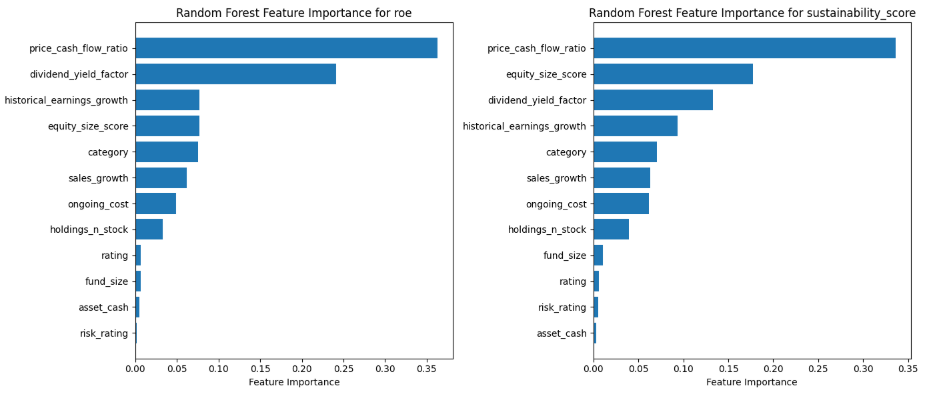
\includegraphics[width=\textwidth]{rffeatureimportance.png}
    \caption{Feature importance plot for the Random Forest model.}
\end{figure}

In the case of Return on Equity (ROE), the plot highlights the price-to-cash flow ratio as the most influential feature, followed by the dividend yield factor and historical earnings growth. These features significantly shape the model's ability to predict ROE, suggesting that financial metrics related to profitability and growth are key drivers of the model's performance. Equity size score and category also play important roles, but their relative importance is lower compared to the leading features.

For the Sustainability Score, the feature importance plot similarly underscores the price-to-cash flow ratio as the dominant variable. Equity size score and dividend yield factor follow closely, indicating that firm size and return metrics are critical in determining sustainability outcomes. The contributions of features such as category and historical earnings growth further enhance the model's predictions, reflecting the complex interplay between financial performance and sustainability indicators.

Overall, these plots highlight the critical role of financial and growth-related variables in predicting both ROE and Sustainability Scores. By focusing on the most influential features, model refinements can be directed toward the areas that yield the highest impact on predictive accuracy.

While the model demonstrates strong results for the Sustainability Score, the higher error in ROE predictions points to potential areas for improvement. Further steps could include refining the feature set, tuning hyper-parameters, or experimenting with alternative regression models to enhance predictive accuracy. Addressing these areas can help reduce the discrepancy between the two targets and improve the overall reliability of the model.  

In conclusion, the Random Forest model shows promising results but exhibits uneven performance across the target variables. With targeted refinements, the model's ability to predict both ROE and Sustainability Score can be enhanced, leading to more accurate and consistent predictions.


%%MRCE Info:
\item Iterate until convergence, so repeat Steps 1 and 2 until \( \mathbf{B} \) and \( \boldsymbol{\Omega} \) stabilise. The convergence criterion can be based on a change in the objective function value and a difference in parameter estimates between iterations.
\end{enumerate}

\noindent Step 1 is a regularised least squares problem with an \( \ell_1 \)-penalty (Lasso) on the elements of \( B \), enforcing sparsity in the regression coefficients. This solution can be obtained by coordinate descent or proximal gradient methods. 

This proof is covered using proximal gradient methods and by combining methodology from Friedman et al. (2008) and Rothman et al. (2007).

Firstly, \ref{B as Omega} can be written as: $\min_{\mathbf{B}} \left\{ f(\mathbf{B}) + \lambda_2 \|\mathbf{B}\|_1 \right\},$
where \( f(\mathbf{B}) \) is the least squares loss term. The proximal gradient method updates \( \mathbf{B} \) iteratively as:

\[
\mathbf{B}^{(t+1)} = \mathbf{S}_{\lambda_2} \left( \mathbf{B}^{(t)} - \eta \nabla f(\mathbf{B}^{(t)}) \right),
\]

\noindent where \( \mathbf{S}_{\lambda_2} = \text{sign}(z) \max(|z| - \lambda_2, 0)\) is the soft-thresholding operator.

Since the proximal gradient method is valid for convex functions with an \( \ell_1 \)-penalty, this proves that the solution can be obtained using proximal gradient descent. \( \blacksquare \)

Step 2 estimates the inverse covariance matrix \( \boldsymbol{\Omega} \), assuming many off-diagonal elements are zero and is solved using the Graphical Lasso algorithm, which is outlined next. The aim of this is to write \ref{Omega as B} in this form of \ref{GL}:

\noindent The key to this is to identify the corresponding terms in both equations, which are:
\begin{itemize}
    \item \(\text{tr} (\mathbf{\Sigma}_R \mathbf{\Omega})\) in MRCE corresponds to \(\text{tr}(\mathbf{S} \mathbf{\Omega})\) in Graphical Lasso.
    \item The log-determinant, \(-\log |\mathbf{\Omega}|\), in MRCE matches Graphical Lasso since maximising \(\log \det \mathbf{\Omega}\) is equivalent to minimising \(-\log |\mathbf{\Omega}|\).
    \item The \(\ell_1\)-penalty, \(\lambda_1 \sum_{j' \neq j} |\omega_{j'j}|\), in MRCE exactly corresponds to \(\lambda \|\mathbf{\Omega}\|_1\) in GLasso.
\end{itemize}

\noindent Thus, by multiplying the entire function by \(-1\), the MRCE formulation becomes:

\[
\max_{\mathbf{\Omega} \succ 0} \left( \log \det (\mathbf{\Omega}) - \text{tr}(\mathbf{\Sigma}_R \mathbf{\Omega}) - \lambda_1 \|\mathbf{\Omega}\|_1 \right),
\]

\noindent which is the Graphical Lasso problem. $\blacksquare$

\noindent The performance of MRCE also depends on the regularisation parameters, which are selected here via cross-validation:
\begin{equation*}
    (\lambda_1^*, \lambda_2^*) = \arg \min_{\lambda_1, \lambda_2} \sum_{k=1}^{K} \| \mathbf{Y}^{(k)} - \mathbf{X}^{(k)} \mathbf{B}_{\lambda_1, \lambda_2}^{(-k)} \|_F^2,
\end{equation*}
where \( \mathbf{Y}^{(k)} \) is the matrix of responses with observations in the \( k \)th fold, \( \mathbf{X}^{(k)} \) is the matrix of predictors of observations in the \( k \)th fold, and \( \mathbf{B}_{\lambda_1, \lambda_2}^{(-k)} \) is the estimated regression coefficient matrix computed with observations outside the \( k \)th fold, 
with tuning parameters \( \lambda_1 \) and \( \lambda_2 \).\cite{rothman2010sparse} 


%% MRCE Advantages:
\noindent MRCE has a few advantages, which are: error correlation incorporation, sparsity and flexibility. By jointly estimating \( \mathbf{B} \) and \( \boldsymbol{\Omega} \), MRCE improves prediction accuracy, especially when responses are highly correlated.
 The $L_1$ penalties encourage sparsity in the regression coefficients and the precision matrix, leading to interpretable models. Finally, MRCE is well-suited for high-dimensional datasets where traditional methods fail.

%% Graphical Lasso

\subsection{Multivariate Graphical Lasso}
The Graphical Lasso (GLasso) is a method which estimates the inverse covariance, or precision, matrix independently of regression models. GLasso achieves sparsity, which is setting off-diagonal elements to zero, by imposing an $L_1$ penalty on the precision matrix, and it solves the following optimisation problem:
\begin{equation}
    \max_{\boldsymbol{\Omega} \succ 0} \left( \log \det (\boldsymbol{\Omega}) - \text{tr}(\mathbf{S}  \boldsymbol{\Omega}) - \lambda \|\boldsymbol{\Omega}\|_1 \right),
\label{GL}
\end{equation}
where \( \mathbf{S}  \) is the empirical covariance matrix, \( \lambda \) is a regularisation parameter, \( \boldsymbol{\Omega}\) is the precision matrix, \( \log \det (\boldsymbol{\Omega}) \) ensures precision matrix positive definiteness and \( \|.\|_1 \) is the $L_1$ penalty.\citep{friedman2008sparse}

GLasso brings conditional independence and computational efficiency. A zero entry \( \boldsymbol{\Omega}_{ij} = 0 \) implies that variables \( i \) and \( j \) are conditionally independent given all other variables. GLasso also uses a blockwise coordinate descent algorithm, making it significantly faster than traditional maximum likelihood estimation methods. Here is the blockwise coordination descent algorithm:

\begin{enumerate}
    \item Start with \( \mathbf{W} = \mathbf{S} + \lambda \mathbf{I} \). The diagonal of \( \mathbf{W} \) remains unchanged in what follows, 
    \item For each \( j = 1,2,\dots, p, 1,2,\dots, p, \dots \), solves \textbf{the lasso problem (2.4)}, which takes as input the inner products \( \mathbf{W}_{11} \) and \( s_{12} \). This gives a \( p - 1 \) vector solution \( \hat{\beta} \). Fill in the corresponding row and column of \( \mathbf{W} \) using \( w_{12} = \mathbf{W}_{11} \hat{\beta} \),
    \item Continue until convergence.\cite{friedman2008sparse}
\end{enumerate}

GLasso was introduced to set up the shrinkage method in the next section, multivariate response covariance estimation. It provides an initial sparse precision matrix estimate, which can be incorporated into its covariance structure estimation. This hybrid approach is beneficial, particularly when responses have strong conditional dependencies.


% More RRRR Theory
\noindent This new objective function is assumed to follow standard OLS, so we can compute  $\hat{\mathbf{B}}(\lambda, r)$ = $\hat{\mathbf{B}}_R$

Before solving this Reduced Rank Regression problem, let us start with the Ridge part.

Ridge is solved using the standard mechanism introduced in the previous section via its closed-form solution: \(\hat{\mathbf{B}}_{\text{ridge}} = (\mathbf{X}^T \mathbf{X} + \lambda \mathbf{I})^{-1} \mathbf{X}^T \mathbf{Y}.\) The standard \( \mathbf{X} \) and \( \mathbf{Y} \) are used instead of \( \mathbf{X^*} \) and \( \mathbf{Y^*} \). This is because, when incorporating ridge into the augmented objective function and solving for the rank constraint (which will be done in the next paragraph), we have not actually solved for ridge.

Now, to solve this augmented objective function,




%% Extra RRRR Theory
The OLS estimate has an orthogonal projection property, which means this new objective function can be decomposed into 2 parts: $
\|\mathbf{Y}^* - \mathbf{X}^* \mathbf{B} \|_F^2 = \|\mathbf{Y}^* - \hat{\mathbf{Y}}^*_R \|_F^2 + \|\hat{\mathbf{Y}}^*_R - \mathbf{X}^* \mathbf{B} \|_F^2
$, where \( \hat{\mathbf{Y}}^*_R = \mathbf{X}^* \hat{\mathbf{B}}^*_R \) denotes the Ridge Regression estimate.\cite{mukherjee2011reduced} The first term of this equation does not involve $\mathbf{B}$ so the objective function can be further simplified into:
\begin{equation*}
    \hat{\mathbf{B}}(\lambda, r) = \arg\min_{\operatorname{rank}(\mathbf{B}) \leq r} ||\hat{\mathbf{Y}}^*_R - \mathbf{X}^* \mathbf{B}||_{F}^2.
\end{equation*}

%% Old RRRR explanation
Reduced Rank Ridge Regression (RRRR) is effective in cases where multiple response variables exhibit intercorrelations, the true coefficient matrix is of a lower rank and where there is high collinearity among predictor variables.\cite{mukherjee2011reduced} Although the true coefficient matrix is not of a lower rank and high collinearity amongst predictor variables has been sorted in pre-processing, the responses have a correlation of \texttt{-0.317}, which needs to be considered.

RRRR considers response intercorrelation when it introduces a low-rank constraint on the coefficient matrix. This will be explained further once the full model has been introduced. RRRR also incorporates a ridge penalty to improve estimation stability when predictors are multi-collinear.\cite{mukherjee2011reduced}

\noindent RRRR estimates the coefficient matrix, \( \mathbf{B} \) by solving:

\[
\mathbf{B}(\lambda, r) = \arg \min_{\mathbf{B}: \text{rank}(\mathbf{B}) \leq r} \|\mathbf{Y} - \mathbf{X} \mathbf{B}\|_F^2 + \lambda \|\mathbf{B}\|_F^2,
\]

\noindent where the constraint \(\text{rank}(\mathbf{B}) \leq r = \text{min}(p,m)\) ensures that \(\mathbf{B}\) has a reduced rank, forcing it to have at most \(r\) independent columns. The $(p,m)$ restriction on $r$ comes from the standard MRR formula:
$\boldsymbol{Y}_{(n \times m)} = \boldsymbol{Z}_{(n \times p)} \, \boldsymbol{\beta}_{(p \times m)} + \boldsymbol{\epsilon}_{(n \times m)}$.

\noindent Intercorrelation between responses is handled by projecting the ridge regression estimate onto a lower-dimensional subspace using singular value decomposition. The estimated response matrix \( \hat{\mathbf{Y}}^*_R \) is decomposed as:
\[
\hat{\mathbf{Y}}^*_R = \sum_{\tau=1}^{Q} \sigma_i \mathbf{u}_i \mathbf{v}_i^T,
\]
\noindent where \( \sigma_i \) are the singular values, and \( \mathbf{u}_i, \mathbf{v}_i \) are the left and right singular vectors, respectively. \cite{mukherjee2011reduced} The best rank-\( r \) approximation to \( \hat{\mathbf{Y}}^*_R \) in the Frobenius norm is obtained by retaining only the first \( r \) singular values and their corresponding singular vectors, ensuring that the estimated responses align with the most prominent singular values. \cite{mukherjee2011reduced} This projection allows RRRR to capture dependencies between responses while filtering out noise from lower-importance dimensions. \cite{mukherjee2011reduced} 

Given the ridge regression solution \( \mathbf{B}_R^* \), the final estimate is obtained as: $\mathbf{B}(\lambda, r) = \mathbf{B}_R^* \mathbf{P}_r$, where \( \mathbf{P}_r \) is the projection onto the first \( r \) principal components of the ridge-estimated response matrix. This transformation captures the shared structure among responses while eliminating noise in less significant dimensions.\cite{mukherjee2011reduced}

\noindent The choice of the rank \( r \) and penalty parameter \( \lambda \) is made through cross-validation:
\[
(\lambda^*, r^*) = \arg \min_{\lambda, r} \sum_{k=1}^{K} \| \mathbf{Y}^{(k)} - \mathbf{X}^{(k)} \mathbf{B}^{(-k)}(\lambda, r) \|_F^2.
\]
This approach is best for a medium-sized dataset, which the equity fund data is, and it balances bias and variance, ensuring optimal performance.

Another way to model response dependencies is through their inverse covariance matrix, which considers the conditional dependencies. This is how Graphical Lasso works.



%Extra on RRRR
RRRR is used in this report over traditional reduced rank regression (RRR) due to the problem the latter brings. Suppose there are 3 responses and 3 predictors, with coefficient matrix:
\[
\mathbf{B} = \begin{bmatrix} 1 & 3 & 0 \\ 3 & 1 & 0 \\ 0 & 0 & 0 \end{bmatrix},
\]
and predictor covariance:
\[
{\Sigma}_X = \begin{bmatrix} 1 & 0.95 & 0 \\ 0.95 & 1 & 0 \\ 0 & 0 & 1 \end{bmatrix}.
\]

\noindent Here, standard RRR fails because it does not consider predictor collinearity. RRRR, by adding ridge regularisation, correctly preserves the relevant structure.\cite{mukherjee2011reduced} Here, the first two predictors are highly correlated with a correlation coefficient of 0.95, while the third predictor is uncorrelated with the first two. This high correlation leads to multicollinearity, which can distort standard regression estimates by making it difficult to separate the contributions of highly correlated predictors.  

Standard reduced rank regression does not take predictor collinearity into account and instead focuses solely on reducing the dimensionality of the coefficient matrix. Because predictors one and two are nearly identical in their information content, standard reduced rank regression may incorrectly attribute too much or too little importance to one predictor over the other, leading to unstable estimates. This issue is particularly problematic when the predictors are highly collinear, as seen in this example, where predictors one and two are strongly correlated.  

Reduced rank ridge regression addresses this issue by incorporating ridge regularization, which adds a penalty to the magnitude of the coefficients in \( \mathbf{B} \). This ridge penalty ensures that the estimates remain stable even when predictors exhibit high multicollinearity. By penalizing large coefficients, reduced rank ridge regression prevents overfitting to specific predictors and encourages a more balanced allocation of influence across correlated predictors.  

In this example, reduced rank ridge regression correctly preserves the low-rank structure of \( \mathbf{B} \) while mitigating the adverse effects of multicollinearity. The trade-off between dimensionality reduction and ridge shrinkage ensures that the model maintains a meaningful representation of the predictor-response relationships while avoiding instability. In contrast, standard reduced rank regression, which does not impose a penalty on large coefficients, may produce an incorrect rank structure due to its inability to handle collinearity effectively.  

This example highlights the key advantage of reduced rank ridge regression in scenarios where predictors are highly correlated. By incorporating ridge regularization, it ensures a more robust estimation of the coefficient matrix, preserving the correct response structure while preventing distortions caused by collinearity.


% Lasso Proof
 The cost function is expanded as before. So, the cost function becomes:
\[
J(\boldsymbol{\beta}) = \mathbf{Y}^\top \mathbf{Y} - 2 \mathbf{Y}^\top \mathbf{X} \boldsymbol{\beta} + \boldsymbol{\beta}^\top \mathbf{X}^\top \mathbf{X} \boldsymbol{\beta} + \lambda \sum_{j=1}^p |\beta_j|
\]

\noindent To minimise \(J(\boldsymbol{\beta})\), compute the derivative (or sub-gradient) with respect to \(\boldsymbol{\beta}\). Since the \(L_1\)-norm \(\|\boldsymbol{\beta}\|_1 = \sum_{j=1}^p |\beta_j|\) is not differentiable at \(\beta_j = 0\), the sub-gradient is used:
\[
\frac{\partial |\beta_j|}{\partial \beta_j} =
\begin{cases}
+1 & \text{if } \beta_j > 0 \\
-1 & \text{if } \beta_j < 0 \\
[-1, +1] & \text{if } \beta_j = 0
\end{cases}
\]

\noindent The derivative of the quadratic term is:
\[
\frac{\partial}{\partial \boldsymbol{\beta}} \|\mathbf{Y} - \mathbf{X}\boldsymbol{\beta}\|_2^2 = -2 \mathbf{X}^\top \mathbf{Y} + 2 \mathbf{X}^\top \mathbf{X} \boldsymbol{\beta}
\]

\noindent Combining these, the sub-gradient of \(J(\boldsymbol{\beta})\) is:
\[
\frac{\partial J(\boldsymbol{\beta})}{\partial \boldsymbol{\beta}} = -2 \mathbf{X}^\top \mathbf{Y} + 2 \mathbf{X}^\top \mathbf{X} \boldsymbol{\beta} + \lambda \mathbf{s}
\]
where \(\mathbf{s} \in \partial \|\boldsymbol{\beta}\|_1\) is the sub-gradient of the \(L_1\)-norm. The sub-gradient is set to zero to find the minimum:
\begin{align*}
-2 \mathbf{X}^\top \mathbf{Y} + 2 \mathbf{X}^\top \mathbf{X} \boldsymbol{\beta} + \lambda \mathbf{s} &= 0 \\
2 \mathbf{X}^\top \mathbf{X} \boldsymbol{\beta} &= 2 \mathbf{X}^\top \mathbf{Y} - \lambda \mathbf{s} \\
\mathbf{X}^\top \mathbf{X} \boldsymbol{\beta} &= \mathbf{X}^\top \mathbf{Y} - \frac{\lambda}{2} \mathbf{s}
\end{align*}


\noindent The presence of \(s\), the sub-gradient of the \(L_1\)-norm, provides the sparsity property of Lasso. Specifically, for \(\beta_j \neq 0\), \(s = \text{sign}(\beta_j)\), which shrinks \(\beta_j\), while for \(\beta_j = 0\), \(s \in [-1, 1]\), allowing coefficients to be exactly zero. $\blacksquare$

% Ridge Proof
This is the cost function Ridge Regression aims to minimise in a different format: 

\[
\|\boldsymbol{Y} - \boldsymbol{X\beta}\|_2^2 + \lambda \|\boldsymbol{\beta}\|_2^2 =
RSS + \lambda \boldsymbol{\beta}^T \boldsymbol{\beta}
\]


\noindent The second equality is expressing the residual sum of squares (RSS) as a matrix, which will be expanded upon and differentiated.

\begin{align*}
RSS + \lambda \boldsymbol{\beta}^T \boldsymbol{\beta} 
    &= (\mathbf{y} - \mathbf{X} \boldsymbol{\beta})^T (\mathbf{y} - \mathbf{X} \boldsymbol{\beta}) + \lambda \boldsymbol{\beta}^T \boldsymbol{\beta} \\
    &= \mathbf{y}^T \mathbf{y} - 2 \boldsymbol{\beta}^T \mathbf{X}^T \mathbf{y} + \boldsymbol{\beta}^T \mathbf{X}^T \mathbf{X} \boldsymbol{\beta} + \lambda \boldsymbol{\beta}^T \boldsymbol{\beta}
\end{align*}

\noindent Take the gradient with respect to $\boldsymbol{\beta}$ and set it to zero for the minimum:

\begin{align*}
-2 \mathbf{X}^T \mathbf{y} + 2 \mathbf{X}^T \mathbf{X} \boldsymbol{\beta} + 2 \lambda \boldsymbol{\beta} &= 0, \\
- \mathbf{X}^T \mathbf{y} + \mathbf{X}^T \mathbf{X} \boldsymbol{\beta} + \lambda \boldsymbol{\beta} &= 0, \\
\mathbf{X}^T \mathbf{X} \boldsymbol{\beta} + \lambda \boldsymbol{\beta} &= \mathbf{X}^T \mathbf{y}, \\
\left( \mathbf{X}^T \mathbf{X} + \lambda \mathbf{I} \right) \boldsymbol{\beta} &= \mathbf{X}^T \mathbf{y}, \\
\boldsymbol{\hat{\beta}}_{\text{Ridge}} &= \left( \mathbf{X}^T \mathbf{X} + \lambda \mathbf{I} \right)^{-1} \mathbf{X}^T \mathbf{y}.
\quad \hfill \blacksquare
\end{align*}

%Previous SM Results
Now, these regression models will be applied to the dataset to see how well the predictors can model the response variables: \texttt{roe} and \texttt{sustainability\_score}. This can be done by using \texttt{family = "mgaussian"} in \texttt{cv.glmnet}. This will consider the correlation between response variables and maintain consistent variable selection, which is the aim of MRR.

Lasso had an ARSR of \texttt{0.737}, Ridge had ARSR of \texttt{0.741} and Group Lasso had an ARSR of \texttt{0.739}. Elastic Net had the lowest ARSR of \texttt{0.736} because of its Lasso and Ridge combination which allows it to handle datasets with both sparsity and high multicollinearity effectively. As a result, it balances feature selection and regularisation, resulting in the lowest ARSR. The feature selection capability of Lasso performs well. However, it was slightly worse than Elastic Net due to its limitations in handling correlated predictors and bias in over-shrinking weaker predictor coefficients. Despite these challenges, Lasso's ARSR suggests that sparsity played a significant role in the dataset.

Group Lasso uses the \( L_{2,1} \) penalty, enforcing sparsity for groups rather than for individual predictors. In this case, its performance was slightly worse than Lasso and Elastic Net due to the reduced flexibility of group-level constraints, which may retain irrelevant groups or eliminate entire groups prematurely. The additional constraints introduced by grouping variables made it less effective when individual feature sparsity was more relevant. The slight increase in ARSR suggests that the grouping strategy did not perfectly align with the data structure. Ridge regression performed the worst among the models, as it applies only an \( L_2 \) penalty, which shrinks all coefficients uniformly toward zero but does not enforce sparsity. Ridge retains all predictors, including irrelevant ones, which can introduce noise and inflate residuals. Additionally, its inability to address sparsity makes it less effective in datasets with many irrelevant predictors. Despite these limitations, Ridge's ability to handle multicollinearity effectively prevents over-fitting, keeping it competitive, albeit at the highest ARSR.

Here is a representation of how the ARSR changed with the $\alpha$ parameter, which controlled how much the $L_1$ and $L_2$ penalties contributed to the model:

\begin{figure}[H]
    \centering
    \includegraphics[height=7.5cm, width=7.5cm]{Alpha vs EN ARSR.pdf}
    \caption{A plot of $\alpha$ vs Elastic Net ARSR}
    \label{fig:alphaelasticnet}
\end{figure}


Tikka et al. (2007) introduced an extension of lasso used in multiple response regression called lasso simultaneous variable selection ($L_2$-SVS). It extends the lasso to account for the relationships across multiple response variables simultaneously. The \(L_2\)-SVS approach minimises the residual error while enforcing sparsity in the solution by penalising the model with a row-wise \(L_2\)-norm combined with an \(L_1\)-norm over the rows of the coefficient matrix. The optimisation problem for \(L_2\)-SVS can be written as:

\[
\min_{\mathbf{W}} \frac{1}{2} \|\mathbf{Y} - \mathbf{X}\mathbf{W}\|_F^2 + \lambda \|\mathbf{W}\|_{1,2},
\]

where: \(\|\mathbf{W}\|_{1,2} = \sum_{j=1}^m \|\mathbf{w}_j\|_2\) is the mixed norm, combining the row-wise \(L_2\)-norm (\(\|\mathbf{w}_j\|_2\)) with an \(L_1\)-penalty. The \(L_2\)-SVS regression model encourages sparsity by driving entire rows of \(\mathbf{W}\) to zero, effectively removing predictors from the model across all responses. This property makes \(L_2\)-SVS particularly effective in scenarios where predictors are expected to be relevant (or irrelevant) across multiple response variables. \(L_2\)-SVS has high prediction and selection accuracy when many input variables are available for model construction.\cite{simila2007input} It is consistently more precise and stable than ridge, and it outperforms lasso, especially when the input variables are highly correlated.\cite{simila2007input} 

\noindent Elastic Net combines the standard Lasso and Ridge penalties:

\[
\min_{\mathbf{W}} \frac{1}{2} \| \mathbf{Y} - \mathbf{X}\mathbf{W} \|_2^2 + \alpha \lambda \|\mathbf{W}\|_1 + (1-\alpha)\lambda \|\mathbf{W}\|_2^2,
\]

\noindent where \(\|\mathbf{W}\|_1 = \sum_{j=1}^m |w_j|\) is the sparsity-inducing penalty, and \(\|\mathbf{W}\|_2^2 = \sum_{j=1}^m w_j^2\) adds the ridge penalty to stabilise the model.


\subsection{Elastic Net}
The Elastic Net uses a convex combination of the penalties of lasso and ridge regression, with the following cost function minimisation:\cite{elasticnet}

\begin{equation*}
    \sum_{i=1}^{n} \left( y_i - \beta_0 - \sum_{j=1}^{p} \beta_j x_{ij} \right)^2 
+ \lambda \alpha \sum_{j=1}^{p} |\beta_j| 
+ \lambda (1 - \alpha) \sum_{j=1}^{p} \beta_j^2
= \text{RSS} + \lambda \alpha \sum_{j=1}^{p} |\beta_j| + \lambda (1 - \alpha) \sum_{j=1}^{p} \beta_j^2
\end{equation*}

\noindent where, $\alpha$ controls the trade-off between the $L_1$ and $L_2$ penalties. It can be proven to minimise its cost function by combining the lasso and ridge proofs previously.

The elastic net regression cost function estimates are the solution to the least squares problem subject to the constraint $\alpha\sum_{j=1}^p |\beta_j| + (1-\alpha)\sum_{j=1}^p \beta_j^2\leq c$, where $\alpha \in [0,1]$. A geometric interpretation of this is a diamond mixed with a circle depending on what $\alpha$ is. $\alpha = 0$ corresponds to ridge regression and $\alpha = 1$ corresponds to lasso regression. Here is how all the shrinkage methods are visually:

\begin{figure}[H]
    \centering
    \includegraphics[width=0.6\textwidth]{elasticnet.png}
    \caption{Geometric Interpretation of Shrinkage Methods  \cite{cfi2024elasticnet}}
    \label{fig:elasticnet}
\end{figure}

\noindent One of the major benefits of the Elastic Net is its grouping effect. This can be derived: 
given data \((\mathbf{y}, \mathbf{X})\) and parameters \(\lambda_1, \lambda_2\),\(\mathbf{y}\), the response, is centred and the predictors \(\mathbf{X}\) are standardised.\cite{elasticnet} Let \(\hat{\beta}(\lambda_1, \lambda_2)\) be the naïve Elastic Net estimate. Suppose that \(\hat{\beta}_i(\lambda_1, \lambda_2) \hat{\beta}_j(\lambda_1, \lambda_2) > 0\). Define:
\[
D_{\lambda_1, \lambda_2}(i, j) = \frac{1}{\|\mathbf{y}\|_1} \left| \hat{\beta}_i(\lambda_1, \lambda_2) - \hat{\beta}_j(\lambda_1, \lambda_2) \right|,
\]
Then:
\[
D_{\lambda_1, \lambda_2}(i, j) \leq \frac{1}{\lambda_2} \sqrt{2(1 - \rho)},
\]
where \(\rho = \mathbf{x}_i^T \mathbf{x}_j\), the sample correlation.

\noindent \(D_{\lambda_1, \lambda_2}(i, j)\) is the difference between the coefficient paths of predictors \(i\) and \(j\).\cite{elasticnet} If \(\mathbf{x}_i\) and \(\mathbf{x}_j\) are highly correlated, the difference between the coefficient paths of predictor \(i\) and predictor \(j\) is almost 0.\cite{elasticnet} The upper bound in the above inequality is a mathematical representation of the grouping effect of the naïve Elastic Net. Only the ridge parameter, $\lambda_2$, is in the grouping effect and not $\lambda_1$ because ridge exhibits this property, unlike lasso.


Another benefit of the Elastic Net is that it retains the variable selection property of Lasso and remains computationally efficient while overcoming its limitation with high-dimensional data.\cite{elasticnet} Elastic Net also handles correlated predictors better by encouraging a group effect in contrast to Lasso, which arbitrarily selects one variable from a group of highly correlated predictors.\cite{elasticnet} Although there is a moderate correlation between some of the predictors, this has mainly been sorted in pre-processing. However, Elastic Net does improve prediction accuracy. In situations where both $L_1$ and $L_2$ penalties are needed, Elastic Net balances the two, enhancing prediction performance than Lasso or Ridge alone.\cite{elasticnet} Finally, the Elastic Net is flexible with tuning. The two regularisation parameters, $\lambda_1$ and $\lambda_2$, allow the model to adjust the degree of sparsity and stability, making the Elastic Net a flexible tool for regression.\cite{elasticnet}

However, it does come with quite a few drawbacks. Its first disadvantage is the complexity of tuning. Tuning the Ridge and Lasso regularisation parameters simultaneously makes Elastic Net computationally more intensive than Lasso or Ridge.\cite{elasticnet} Over-shrinkage can be a consequence of improperly chosen regularisation parameters, which can result in biased coefficient estimates.\cite{elasticnet} The next issue is
interpretability in group selection. The grouping effect, while useful, can also select irrelevant predictors if they are highly correlated with relevant ones, making interpretation more difficult.\cite{elasticnet} The final issue of Elastic Net is its dependence on standardisation. Elastic Net assumes predictors have been standardised, as the penalties are applied based on the scale of the variables.\cite{elasticnet}

\subsection{Exploratory Data Analysis}
\begin{lstlisting}[language=R, breaklines=true, basicstyle=\ttfamily\small, columns=fullflexible]
data <- read.csv('clean.csv')
data$equity_category <- as.factor(data$equity_category)
rating <- as.factor(data$rating)
risk_rating <- as.factor(data$risk_rating)

head(data)     
table(rowSums(is.na(data)))

clean_data <- data[rowSums(is.na(data)) < 3, ]
str(clean_data)
     
install.packages("ranger")
library(ranger)
library(dplyr)

# Impute missing continuous variables using lm
impute_continuous_lm <- function(data, column) {
  # Train a linear model excluding rows with NA in the column
  lm_model <- lm(as.formula(paste(column, "~ .")), data = data, na.action = na.exclude)

  # Predict missing values
  missing_indices <- which(is.na(data[[column]]))
  if (length(missing_indices) > 0) {
    predictions <- predict(lm_model, newdata = data[missing_indices, ])

    # Replace NA values with predictions
    data[[column]][missing_indices] <- predictions
  }

  return(data)
}

# Function to impute missing categorical variables using ranger
impute_categorical_rf <- function(data, column) {
  # Train a Random Forest classification model excluding rows with NA in the column
  rf_model <- ranger(
    formula = as.formula(paste(column, "~ .")),
    data = data[!is.na(data[[column]]), ],
    na.action = "na.omit",
    classification = TRUE
  )

  # Predict missing values
  missing_indices <- which(is.na(data[[column]]))
  if (length(missing_indices) > 0) {
    predictions <- predict(
      rf_model,
      data = data[missing_indices, ]
    )$predictions

    # Replace NA values with predictions
    data[[column]][missing_indices] <- predictions
  }

  return(data)
}

# Identify numerical and categorical columns
numerical_columns <- names(clean_data)[sapply(clean_data, is.numeric)]
categorical_columns <- names(clean_data)[sapply(clean_data, is.factor)]

# Impute missing values for numerical columns using lm
for (col in numerical_columns) {
  if (any(is.na(clean_data[[col]]))) {
    clean_data <- impute_continuous_lm(clean_data, col)
  }
}

# Impute missing values for categorical columns using ranger
for (col in categorical_columns) {
  if (any(is.na(clean_data[[col]]))) {
    clean_data <- impute_categorical_rf(clean_data, col)
  }
}

# Verify that no missing values remain
if (any(is.na(clean_data))) {
  stop("There are still NA values in the data!")
} else {
  print("All missing values have been successfully imputed!")
}

summary(clean_data)
# head(clean_data)
any(is.na(clean_data))

clean_data$holdings_n_stock <- round(clean_data$holdings_n_stock) # holdings_n_stock is an integer value
price_cash_flow_ratio, digits = 3) # keeps it consistent with actual values

\end{lstlisting}

\subsection{Multiple Response Regression}
\begin{lstlisting}[language=R, breaklines=true, basicstyle=\ttfamily\small, columns=fullflexible]

# Frequency encode the categorical variables
rating_counts <- table(data$rating)
data$rating_encoded <- as.numeric(rating_counts[data$rating])

risk_rating_counts <- table(data$risk_rating)
data$risk_rating_encoded <- as.numeric(risk_rating_counts[data$risk_rating])

equity_category_counts <- table(data$equity_category)
data$equity_category_encoded <- as.numeric(equity_category_counts[data$equity_category])

data <- data[, setdiff(names(data), c("rating", "risk_rating", "equity_category"))]
dim(data)


multi_model <- lm(cbind(roe, sustainability_score)~., data = data)

calculate_nrmse <- function(model, data) {
  residuals_matrix <- residuals(model)

  if (is.null(residuals_matrix) || ncol(as.matrix(residuals_matrix)) == 0) {
    stop("Residuals matrix is NULL or has zero dimensions.")
  }

  # Calculate RMSE for each response
  rmse_per_response <- apply(as.matrix(residuals_matrix), 2, function(residuals) {
    sqrt(mean(residuals^2))
  })

  # Normalize RMSE by the standard deviation of each response variable
  response_vars <- c("roe", "sustainability_score")
  std_devs <- apply(data[, response_vars], 2, function(column) {
    sd(column, na.rm = TRUE)
  })

  nrmse <- sum(rmse_per_response / std_devs) / length(std_devs)  # Aggregate across responses
  return(nrmse)
}
multi_model <- lm(cbind(roe, sustainability_score)~., data = data)
print(calculate_nrmse(multi_model, data))

add_predictors <- function(data, response_vars, selected_predictors, remaining_predictors) {
  metrics <- c()
  candidate_models <- list()

  for (predictor in remaining_predictors) {
    formula <- as.formula(
      paste0("cbind(", paste(response_vars, collapse = ", "), ") ~ ",
             paste(c(selected_predictors, predictor), collapse = " + "))
    )
    tryCatch({
      model <- lm(formula, data = data)
      metric <- calculate_nrmse(model, data)
      metrics <- c(metrics, metric)
      candidate_models[[predictor]] <- model
    }, error = function(e) {
      metrics <- c(metrics, NA)
      candidate_models[[predictor]] <- NULL
    })
  }

  return(list(metrics = metrics, candidate_models = candidate_models))
}

remove_predictors <- function(data, response_vars, selected_predictors) {
  metrics <- c()
  candidate_models <- list()

  for (predictor in selected_predictors) {
    remaining_predictors <- setdiff(selected_predictors, predictor)

    if (length(remaining_predictors) > 0) {
      formula <- as.formula(
        paste0("cbind(", paste(response_vars, collapse = ", "), ") ~ ",
               paste(remaining_predictors, collapse = " + "))
      )
      tryCatch({
        model <- lm(formula, data = data)
        metric <- calculate_nrmse(model, data)
        metrics <- c(metrics, metric)
        candidate_models[[predictor]] <- model
      }, error = function(e) {
        metrics <- c(metrics, NA)
        candidate_models[[predictor]] <- NULL
      })
    }
  }

  return(list(metrics = metrics, candidate_models = candidate_models))
}


# cleaner function
stepwise_multivariate <- function(data, method = "stepwise") {
  response_vars <- c("roe", "sustainability_score")
  predictors <- setdiff(names(data), response_vars)
  selected_predictors <- if (method == "forward") c() else predictors
  remaining_predictors <- if (method == "forward") predictors else c()
  best_model <- NULL
  best_metric <- Inf  # Initialize best nRMSE (lower is better)

  repeat {
    metrics <- c()
    candidate_models <- list()

    # Forward Step: Try adding predictors
    if (method == "forward" || method == "stepwise") {
      forward_results <- add_predictors(data, response_vars, selected_predictors, remaining_predictors)
      metrics <- c(metrics, forward_results$metrics)
      candidate_models <- c(candidate_models, forward_results$candidate_models)
    }

    # Backward Step: Try removing predictors
    if (method == "backward" || method == "stepwise") {
      backward_results <- remove_predictors(data, response_vars, selected_predictors)
      metrics <- c(metrics, backward_results$metrics)
      candidate_models <- c(candidate_models, backward_results$candidate_models)
    }

    # Handle cases where no valid models are generated
    if (length(metrics) == 0 || all(is.na(metrics))) {
      cat("No valid predictors to add or remove. Stopping selection.\n")
      break
    }

    # Select the best candidate model
    valid_metrics <- which(!is.na(metrics) & is.finite(metrics))
    if (length(valid_metrics) == 0) {
      cat("No valid models due to NA or Inf values. Stopping selection.\n")
      break
    }

    best_candidate_index <- valid_metrics[which.min(metrics[valid_metrics])]
    best_candidate_metric <- metrics[best_candidate_index]
    best_candidate_predictor <- names(candidate_models)[best_candidate_index]
    best_candidate_model <- candidate_models[[best_candidate_predictor]]

    # Stop if no improvement
    if (best_candidate_metric >= best_metric) {
      cat("No improvement. Stopping selection.\n")
      break
    }

    # Update the best model and metric
    best_model <- best_candidate_model
    best_metric <- best_candidate_metric

    # Update selected/remaining predictors
    if (method == "forward" || (method == "stepwise" && best_candidate_predictor %in% remaining_predictors)) {
      selected_predictors <- c(selected_predictors, best_candidate_predictor)
      remaining_predictors <- setdiff(remaining_predictors, best_candidate_predictor)
    } else if (method == "backward" || (method == "stepwise" && best_candidate_predictor %in% selected_predictors)) {
      selected_predictors <- setdiff(selected_predictors, best_candidate_predictor)
      remaining_predictors <- c(remaining_predictors, best_candidate_predictor)
    }

    # Debugging Output
    cat("Selected Predictors:", paste(selected_predictors, collapse = ", "), "\n")
    cat("Current nRMSE:", best_metric, "\n")
  }

  return(list(model = best_model, metric = best_metric, predictors = selected_predictors))
}

backward_result <- stepwise_multivariate(data, method = "backward")
nrmse_values <- calculate_nrmse(backward_result$model, data)
print(nrmse_values)

null_model <- lm(cbind(roe, sustainability_score) ~ 1, data = data)

forward_result <- stepwise_multivariate(data, method = "forward")
forward_result
summary(forward_result$model)
cat("Best Metric:", forward_result$metric, "\n")

bidirectional_result <- stepwise_multivariate(data, method = "stepwise")
nrmse_values <- calculate_nrmse(bidirectional_result$model, data)

# Including Interaction Terms
generate_interaction_terms <- function(data, predictors) {
  for (i in 1:(length(predictors) - 1)) {
    for (j in (i + 1):length(predictors)) {
      interaction_name <- paste0(predictors[i], "_x_", predictors[j])
      data[[interaction_name]] <- data[[predictors[i]]] * data[[predictors[j]]]
    }
  }
  return(data)
}
predictors <- setdiff(names(data), c("roe", "sustainability_score"))
data_interaction <- generate_interaction_terms(data, predictors)

bidirectional_result <- stepwise_multivariate(data_interaction, method = "stepwise")
nrmse_values <- calculate_nrmse(bidirectional_result$model, data_interaction)
print(nrmse_values)

# Generate Polynomial Terms
generate_polynomial_terms <- function(data, predictors, degree = 2) {
  for (predictor in predictors) {
    for (d in 2:degree) {
      term_name <- paste0(predictor, "_degree_", d)
      data[[term_name]] <- data[[predictor]]^d
    }
  }
  return(data)
}

# Apply Polynomial Terms
predictors <- setdiff(names(data), c("roe", "sustainability_score"))
data_nonlinear <- generate_polynomial_terms(data, predictors, degree = 3)

# Perform Stepwise Selection
result <- stepwise_multivariate(data_nonlinear, method = "stepwise")
nrmse_values <- calculate_nrmse(result$model, data_nonlinear)
print(nrmse_values)
print("Selected Predictors:")
print(result$predictors)

# Predict values for the same dataset (or a new dataset)
predicted_values <- predict(forward_result$model, newdata = data)

\end{lstlisting}

\subsection{Shrinkage Methods}

\begin{lstlisting}[language=R, breaklines=true, basicstyle=\ttfamily\small, columns=fullflexible]
install.packages("glmnet")
install.packages("caret")
install.packages("ggplot2")
install.packages("grpreg")  # Install the group lasso package

library(glmnet)
library(caret)
library(ggplot2)
library(grpreg)

# Load and preprocess the data
data <- read.csv("C:/Users/raula/OneDrive/Documents/Durham/4th Year/Project/Code/Datasets/clean.csv")
str(data)

# Frequency encode the categorical variables
rating_counts <- table(data$rating)
data$rating_encoded <- as.numeric(rating_counts[data$rating])

risk_rating_counts <- table(data$risk_rating)
data$risk_rating_encoded <- as.numeric(risk_rating_counts[data$risk_rating])

equity_category_counts <- table(data$equity_category)
data$equity_category_encoded <- as.numeric(equity_category_counts[data$equity_category])

data$holdings_n_stock <- as.numeric(data$holdings_n_stock)

# Drop original categorical variables
data <- data[, setdiff(names(data), c("rating", "risk_rating", "equity_category"))]
str(data)

# Define predictors and response
response_vars <- c("roe", "sustainability_score")  # Multivariate responses
predictor_vars <- setdiff(names(data), response_vars)  # All other columns are predictors

# Split data into training and test sets
set.seed(40)
train_index <- sample(seq_len(nrow(data)), size = 0.8 * nrow(data))
train_data <- data[train_index, ]
test_data <- data[-train_index, ]

# Scale predictors and responses
X_train <- scale(as.matrix(train_data[, predictor_vars]))
Y_train <- scale(as.matrix(train_data[, response_vars]))
X_test <- scale(as.matrix(test_data[, predictor_vars]), center = attr(X_train, "scaled:center"), scale = attr(X_train, "scaled:scale"))
Y_test <- scale(as.matrix(test_data[, response_vars]), center = attr(Y_train, "scaled:center"), scale = attr(Y_train, "scaled:scale"))


# Check data structure
cat("Dimensions of X_train:", dim(X_train), "\n")
cat("Dimensions of Y_train:", dim(Y_train), "\n")
cat("Any NA in X_train:", any(is.na(X_train)), "\n")
cat("Any NA in Y_train:", any(is.na(Y_train)), "\n")

# Function to calculate NRMSE for multivariate responses
calculate_nrmse <- function(predictions, actual_data) {
  residuals <- actual_data - predictions
  rmse_per_response <- apply(residuals, 2, function(residuals_col) {
    sqrt(mean(residuals_col^2))
  })
  std_devs <- apply(actual_data, 2, sd, na.rm = TRUE)
  nrmse <- mean(rmse_per_response / std_devs)  # Average NRMSE across all responses
  return(nrmse)
}

# Function to fit models and calculate NRMSE for multivariate regression
fit_and_evaluate <- function(alpha_value, x, y) {
  cv_model <- cv.glmnet(x = x, y = y, family = "mgaussian", alpha = alpha_value)
  lambda_min <- cv_model$lambda.min
  predictions <- predict(cv_model, s = lambda_min, newx = x)[,, 1]
  nrmse <- calculate_nrmse(predictions, y)
  return(list(lambda = lambda_min, nrmse = nrmse, model = cv_model))
}

# Lasso Regression (alpha = 1)
cat("Running Lasso Regression...\n")
lasso_results <- fit_and_evaluate(alpha_value = 1, x = X_train, y = Y_train)
cat("Lasso NRMSE (Train):", lasso_results$nrmse, "\n")
lasso_test_predictions <- predict(lasso_results$model, s = lasso_results$lambda, newx = X_test)[,, 1]
cat("Lasso NRMSE (Test):", calculate_nrmse(lasso_test_predictions, Y_test), "\n")

# Ridge Regression (alpha = 0)
cat("Running Ridge Regression...\n")
ridge_results <- fit_and_evaluate(alpha_value = 0, x = X_train, y = Y_train)
cat("Ridge NRMSE (Train):", ridge_results$nrmse, "\n")
ridge_test_predictions <- predict(ridge_results$model, s = ridge_results$lambda, newx = X_test)[,, 1]
cat("Ridge NRMSE (Test):", calculate_nrmse(ridge_test_predictions, Y_test), "\n")

# Elastic Net Regression (alpha tuning)
cat("Tuning Elastic Net...\n")
alpha_values <- seq(0.1, 0.9, by = 0.1)  # More granular alpha values
elastic_results <- data.frame(alpha = numeric(), lambda = numeric(), train_nrmse = numeric(), test_nrmse = numeric())

for (alpha in alpha_values) {
  result <- fit_and_evaluate(alpha_value = alpha, x = X_train, y = Y_train)
  elastic_test_predictions <- predict(result$model, s = result$lambda, newx = X_test)[,, 1]
  elastic_results <- rbind(elastic_results, data.frame(
    alpha = alpha,
    lambda = result$lambda,
    train_nrmse = result$nrmse,
    test_nrmse = calculate_nrmse(elastic_test_predictions, Y_test)
  ))
}

# Find the best alpha
best_elastic <- elastic_results[which.min(elastic_results$test_nrmse), ]
cat("Best Elastic Net Alpha:", best_elastic$alpha, "\n")
cat("Best Elastic Net Lambda:", best_elastic$lambda, "\n")
cat("Best Elastic Net NRMSE (Train):", best_elastic$train_nrmse, "\n")
cat("Best Elastic Net NRMSE (Test):", best_elastic$test_nrmse, "\n")

# Plot Elastic Net Results
ggplot(elastic_results, aes(x = alpha, y = test_nrmse)) +
  geom_line() +
  geom_point() +
  labs(title = "Elastic Net ARSR vs Alpha", x = "Alpha", y = "Test NRMSE") +
  theme_minimal()

# Group Lasso
cat("Running Group Lasso...\n")

# Define groups (e.g., group predictors by domain knowledge or categories)
groups <- rep(1:length(predictor_vars), each = 1)  # Example: Each predictor is its own group
group_lasso_model <- cv.grpreg(X_train, Y_train, group = groups, penalty = "grLasso")

# Best lambda
group_lambda_min <- group_lasso_model$lambda.min

# Predict and evaluate
group_lasso_predictions <- predict(group_lasso_model, X_test, lambda = group_lambda_min)
group_lasso_nrmse <- calculate_nrmse(group_lasso_predictions, Y_test)
cat("Group Lasso NRMSE (Test):", group_lasso_nrmse, "\n")

# Model Comparison
cat("Model Comparison:\n")
cat("Lasso NRMSE (Test):", calculate_nrmse(lasso_test_predictions, Y_test), "\n")
cat("Ridge NRMSE (Test):", calculate_nrmse(ridge_test_predictions, Y_test), "\n")
cat("Elastic Net NRMSE (Test):", best_elastic$test_nrmse, "\n")
cat("Group Lasso NRMSE (Test):", group_lasso_nrmse, "\n")

\end{lstlisting}

\subsection{Random Forest Regression}
\subsection{XG Gradient Boosting}
\subsection{Neural Networks}

